\documentclass[11pt,a4paper]{article}

% Encoding and language
\usepackage[utf8]{inputenc}
\usepackage[T1]{fontenc}
\usepackage[english]{babel}

% Page geometry
\usepackage[margin=2.5cm]{geometry}

% Math
\usepackage{amsmath, amssymb, amsthm, mathtools}

% Tables
\usepackage{booktabs}
\usepackage{array}

% Graphics
\usepackage{graphicx}
\graphicspath{{figures/}}
\usepackage{float}

% Hyperlinks
\usepackage{xcolor}
\usepackage[colorlinks=true,
            linkcolor=blue!50!black,
            citecolor=blue!50!black,
            urlcolor=blue!50!black]{hyperref}

% Bibliography
\usepackage[numbers, sort&compress]{natbib}
\bibliographystyle{plainnat}

% Typography
\usepackage{microtype}

% Title
\title{Arithmetic structure of the standard genetic code}
\author{Ruslan Khafizov}
\date{\today\\[1ex]
\small Preprint DOI:~\href{https://doi.org/10.5281/zenodo.20751290}{10.5281/zenodo.20751290}}

\begin{document}

\maketitle

\begin{abstract}
The standard genetic code is near-universal and stable over
evolutionary time, motivating study of its arithmetic properties. We analyze proton and neutron counts of the encoded amino acids (free neutral forms) across $33$ codon groups constructed from two natural grouping systems: the Rumer partition by family degeneracy and the three chemical axes of the third codon position (Keto/Amino, Strong/Weak, Purine/Pyrimidine). Excluding the three stop
codons and the initiator $\mathrm{ATG}$ leaves $60$ codons whose group sums
determine an arithmetic structure modulo~$37$. Neutron counts reach
the $37$-lattice, whereas necessarily even proton counts, barred
from odd multiples of $37$, fall one below them: globally, and in
the single tryptophan/isoleucine pair carrying the Keto/Amino
asymmetry, with differences $37$ and $36$. The Keto/Amino balances
and global conditions yield separate neutron and proton equations
modulo~$37$, the former containing $111 = 3 \cdot 37$; since
$\gcd(4, 37) = 1$, these equations fix a unique minimal non-negative
integer assignment for the four service codons, after which the
regularities form a connected family of identities and
divisibilities. Across $27$ NCBI translation tables, this
combination occurs only in the standard code and its exact
codon-to-amino-acid equivalent; deterministic controls show
divisibilities concentrated in third-position groupings, with $37$
standing out among tested prime moduli. Under a random-code null, the observed values of several arithmetic features of this structure fall in the far tails of their Monte Carlo null distributions.
Throughout, the regularities are properties of codon-group sums,
not individual amino acids, and depend jointly on codon degeneracy
and nucleon composition.
\end{abstract}

\tableofcontents

\section{Introduction}
\label{sec:introduction}

The genetic code is one of the most ancient and
conserved molecular features of cellular organisms.
Its near-complete universality across the known
domains of life, and the limited scope of variation
in the known alternative codes, indicate that the
basic structure of the standard code was already
established at the early stages of biological
evolution. Any organizational regularities present in its arithmetic structure therefore require precise analysis as one of the few potential sources of information about the early stages of life.

The arithmetic structure of the standard genetic code has been studied since shortly after its decipherment. Yu.~B.~Rumer~\cite{rumer1966,rumer1968} introduced the partition of the $64$ codons into two classes of $32$ codons each, Octet~I (the eight four-fold degenerate families) and Octet~II (the remaining codons), related by the involution $R = (\mathrm{T} \leftrightarrow \mathrm{G}, \mathrm{C} \leftrightarrow \mathrm{A})$. Shcherbak and Makukov~\cite{makukov2013} observed that the number $37$ plays a recurrent role in the arithmetic of the code, appearing as a divisor of amino acid nucleon sums across various groupings of codons. Panov and Filatov~\cite{panov2024} revisited this analysis, introducing the per-codon counting rule, which forms the methodological basis of the present study.

The present analysis uses the proton and neutron counts of the twenty canonical amino acids in their free neutral forms under the most-abundant-isotope convention; once these conventions are fixed, the counts are uniquely determined. These quantities are considered together with two natural grouping systems defined independently of the nucleon arithmetic. The first is the Rumer partition. The second is
given by the three chemical axes of the third codon
position --- Keto/Amino, Strong/Weak, and
Purine/Pyrimidine --- which exhaust the partitions
of the four nucleotide bases into two pairs and
correspond to the functional-group, hydrogen-bond,
and ring-topology dichotomies of nucleobase
chemistry.

The present work shows that within this framework
the arithmetic regularities of the standard genetic
code organize into a connected family of identities
and divisibilities. The analysis traces this
connected structure to a small number of empirical
properties of the standard code. The same arithmetic criteria are then applied to all $27$ NCBI
translation tables. Among them, the tested combination of structural
regularities occurs only in the standard genetic code table and in its
exact equivalent with respect to codon-to-amino-acid mapping. The specificity of the structure is examined further by deterministic controls, which test its dependence on the third codon position, on the modulus, and on the molecular representation of the amino acids, and by a Monte Carlo test against an explicit random-code null model.

The analysis is divided into three levels. The principal regularities are established at a parametrization-independent level, at which the three stop codons and $\mathrm{ATG}$ in its initiator role are excluded and only the remaining $60$ codons are summed; these are the central results of the paper, and they involve no assigned values. To obtain sums for the complete table of $64$ codons, however, the four service codons must be given some nucleon contributions. The second level is the naive reading (Key~0), in which the stop codons are assigned zero and $\mathrm{ATG}$ is counted as methionine. Assigning zero is also a choice of value, not the absence of one. The third level is the symmetrization (Key~1), in which the four
service codons carry derived nucleon contributions. Key~1 does not
establish the parametrization-independent core of the structure: that
core is already present in sums over the $60$ codons remaining after
the service codons are excluded. The role of Key~1 is to show how the
structure extends to the complete table, taking into account the fixed
distribution of the service codons across the groups in the standard
code. For the chosen
symmetry conditions, these contributions are determined as the unique
minimal non-negative integer solution of the corresponding system
(Section~\ref{sec:results}), and the resulting regularities are
consequences of that solution.

Assigning values to the service codons is a formal device for treating
the arithmetic of the complete table as a single object; neither the
assigned values nor the sums that include them are given a physical
interpretation.

\section{Methods}
\label{sec:methods}

This section defines the nucleon parameters, the codon
group systematics, and the parametrizations of service
codons used throughout the analysis, together with the
computed datasets supporting it.

\subsection{Nucleon composition of amino acids}
\label{sec:composition}

Throughout this work, each of the twenty canonical amino acids is
represented as a free neutral amino acid molecule (not as a residue in
a peptide chain), with its molecular formula retrieved from the
\textsc{PubChem} compound database~\cite{kim2023}. From this formula,
we compute four integer quantities that characterize the nucleon
content of the molecule. Below, $Q(a)$ denotes any of the four
quantities $T$, $P$, $N$, or $\Delta$ for one molecule of amino
acid~$a$. The sensitivity of the results to this choice of molecular
representation is examined in
Section~\ref{sec:discussion-controls}.

The proton count $P$ is defined from the elemental composition of the
molecular formula as
\[
P = \sum_E n_E Z_E,
\]
where $n_E$ is the number of atoms of element $E$ in the formula and
$Z_E$ is its atomic number. The atomic numbers used are
$Z(\mathrm{H}) = 1$, $Z(\mathrm{C}) = 6$, $Z(\mathrm{N}) = 7$,
$Z(\mathrm{O}) = 8$ and $Z(\mathrm{S}) = 16$.

The neutron count $N$ is computed by assigning each element its most
abundant naturally occurring stable isotope, using the terrestrial
isotopic compositions evaluated by IUPAC~\cite{berglund2011}.
Accordingly, we use $^{1}\mathrm{H}$, $^{12}\mathrm{C}$,
$^{14}\mathrm{N}$, $^{16}\mathrm{O}$ and $^{32}\mathrm{S}$. The total
neutron count is
\[
N = \sum_E n_E (A_E - Z_E),
\]
where $A_E$ is the mass number of the selected isotope of element $E$.

The total nucleon count $T$ and the proton--neutron difference
$\Delta$ are defined as
\[
T = P + N, \qquad \Delta = P - N.
\]
Both quantities are integers by construction. Under the isotope
assumptions above, hydrogen is the only element contributing to
$\Delta$, since all other isotopes used have equal numbers of protons
and neutrons. Consequently, $\Delta$ is numerically equal to the number of hydrogen
atoms in the molecule and, in particular, $\Delta \geq 0$ for each of
the twenty canonical amino acids. By linearity, the same identity
holds for any sum of canonical amino-acid contributions and, in
particular, for all group sums over the service-excluded pool
(Section~\ref{sec:genetic-code}).

To avoid a notational collision, we use uppercase $\Delta$ exclusively
for the proton--neutron imbalance of a single molecule or codon group,
and reserve lowercase $\delta$ for pairwise differences between the
molecular quantities of two amino acids (for example, $\delta P=P_i-P_j$
between two amino acids
$i$ and $j$). When both amino acids are identified explicitly, their
labels are placed in parentheses:
\[
\delta Q(a,b)=Q(a)-Q(b).
\]

We emphasize that $P$, $N$, $T$ and $\Delta$ are not measured
molecular masses. They are exact integer quantities derived from
elemental composition, and all arithmetic identities reported in this
study are exact integer relations rather than artifacts of rounding
approximate molecular masses.

The nucleon values for all twenty canonical amino acids are collected
in the input dataset \texttt{amino\_acids\_nucleons.csv}, with one
row per amino acid and columns for $P$, $N$, $T$ and $\Delta$. From
this table we compute three companion datasets of pairwise absolute
differences: \texttt{amino\_acids\_proton\_differences.csv},
\texttt{amino\_acids\_neutron\_differences.csv} and
\texttt{amino\_acids\_nucleon\_differences.csv}. For any pair of amino
acids $(i, j)$ we write $\delta P = P_i - P_j$ and analogously for
$N$ and $T$. Each file groups all $\binom{20}{2} = 190$ unordered pairs $(i,j)$
by the corresponding absolute difference $|\delta P(i,j)|$,
$|\delta N(i,j)|$, or $|\delta T(i,j)|$.

All subsequent nucleon computations for codon groups reduce, by
linearity, to sums of the per-amino-acid values tabulated in
\texttt{amino\_acids\_nucleons.csv}, weighted by the multiplicities of
the corresponding codons. Where service codons are included, their
contributions are determined by the chosen parametrization
(Section~\ref{sec:parametrization}).

\subsection{Genetic code structure}
\label{sec:genetic-code}

The standard genetic code maps the $64$ codons of the four-letter
nucleotide alphabet $\{\mathrm{A}, \mathrm{T}, \mathrm{G}, \mathrm{C}\}$
onto the twenty canonical amino acids and a translation-termination
signal. Throughout this paper, we use DNA notation (with thymine
$\mathrm{T}$ rather than uracil $\mathrm{U}$) and adopt the codon
assignments of The Standard Code (NCBI translation
table~1)~\cite{ncbi2024geneticcodes}. The three codons $\mathrm{TAA}$,
$\mathrm{TAG}$ and $\mathrm{TGA}$ act as stop signals, whereas
$\mathrm{ATG}$ encodes methionine and serves as the canonical
translation-initiation signal. For the purposes of the present
arithmetic analysis, these four codons --- the three stop codons and
$\mathrm{ATG}$ in its initiator role --- are referred to as
\emph{service codons}. Among possible initiation codons, $\mathrm{ATG}$
is predominant. Its RNA equivalent $\mathrm{AUG}$ is the only one of
them fully complementary to the $\mathrm{CAU}$ anticodon of the
initiator methionine tRNA. In the present analysis, $\mathrm{ATG}$
represents the initiation function; this analytical convention does not
exclude initiation from other codons.

Let the complete set of $64$ codons be
\[
\mathcal{C}_{64}
=
\{\mathrm{A},\mathrm{T},\mathrm{G},\mathrm{C}\}^{3},
\]
and let the four service codons form the set
\[
\mathcal{S}
=
\{\mathrm{ATG},\mathrm{TAA},\mathrm{TAG},\mathrm{TGA}\}.
\]
The \emph{service-codon-excluded 60-codon pool} is then defined as
\[
\mathcal{C}_{\mathrm{SE}}
=
\mathcal{C}_{64}\setminus\mathcal{S},
\]
with $|\mathcal{C}_{\mathrm{SE}}|=60$. Every codon belonging to
$\mathcal{C}_{\mathrm{SE}}$ is counted according to its standard
amino-acid assignment. Because $\mathrm{ATG}$ is the sole methionine codon,
$\mathcal{C}_{\mathrm{SE}}$ contains codons for nineteen canonical
amino acids; methionine is absent from this pool. The full codon-to-product mapping is provided
in the dataset \texttt{genetic\_code\_codons.csv}.

By a codon family, we mean the set of four codons sharing the same
first two bases and having an arbitrary third-position base, denoted
by $\mathrm{N}$. A structural property of the standard code, first
identified by Rumer~\cite{rumer1966,rumer1968}, is the partition of
the $64$ codons into two halves of $32$ codons each, distinguished
by the degeneracy pattern of the third codon position. The first
half, which we denote \emph{Octet~I}, consists of the eight codon
families in which all four third-position nucleotides encode the
same amino acid. These fully four-fold degenerate families are
$\mathrm{GCN}$ (Ala), $\mathrm{CGN}$ (Arg), $\mathrm{GGN}$ (Gly),
$\mathrm{CCN}$ (Pro), $\mathrm{ACN}$ (Thr), $\mathrm{GTN}$ (Val),
$\mathrm{CTN}$ (Leu) and $\mathrm{TCN}$ (Ser). The second half,
denoted \emph{Octet~II}, consists of the remaining eight codon
families, in which the third-position nucleotide affects the encoded
product. Every service codon of the standard code belongs to
Octet~II and carries a purine ($\mathrm{A}$ or $\mathrm{G}$) at the
third position.

The Rumer partition is not an analytical construct introduced in the
present work but a structural feature of the code itself. It reflects
both the qualitative distinction between fully and partially
degenerate codon families and the quantitative fact that these two
classes have equal cardinality: each contains eight families and
thirty-two codons. Because Octet~I contains no service codons, all
nucleon quantities computed over Octet~I are independent of any
parametrization of start and stop signals and are determined solely by
the nucleon content of the encoded amino acids. The same property
holds, for a separate reason, for any codon group whose third-position
nucleotide is restricted to pyrimidines (cytosine or thymine), since
all four service codons of the standard code carry a purine at the
third position. Full four-fold degeneracy and a purine-free third
position are two distinct structural conditions, but both have the
same consequence: nucleon quantities over the corresponding groups
are fixed by their amino-acid composition and provide
parametrization-independent reference values for the arithmetic
identities of Section~\ref{sec:results}.

A further structural property of the Rumer partition, introduced by
Rumer~\cite{rumer1968}, is that the two octets are related by a simple
permutation of the nucleotide alphabet. Under the transformation
\[
R =
(\mathrm{T} \leftrightarrow \mathrm{G},\;
 \mathrm{C} \leftrightarrow \mathrm{A}),
\]
each codon family of Octet~I is mapped to a codon family of Octet~II,
and vice versa. This transformation, known as the Rumer
transformation, rearranges the partition but does not preserve the
amino acids encoded by individual codons.

Taken together, the four-fold degeneracy pattern and the Rumer
transformation identify the Octet~I / Octet~II partition as a natural
structural division of the standard code, independent of the nucleon
arithmetic. In the present work, this division is used as a reference
partition over which nucleon quantities are computed and compared.

The codon table (Figure~\ref{fig:codon-table}) is displayed with its
axes in the base ordering $C,G,T,A$, which is also the default ordering
of the accompanying visualizer. This ordering has two
justifications. Chemically, it was introduced by
Rumer~\cite{rumer1968} on the basis of base type and the number
of hydrogen bonds in the canonical base pair. The sequence $C,G,T,A$
alternates pyrimidines and purines,
while within each of these classes the member of the Strong pair
$\{\mathrm{C},\mathrm{G}\}$ precedes the member of the Weak pair
$\{\mathrm{T},\mathrm{A}\}$: $\mathrm{C}$ precedes $\mathrm{T}$
among the pyrimidines, and $\mathrm{G}$ precedes $\mathrm{A}$ among
the purines. Geometrically, as shown by Panov and
Filatov~\cite{panov2024}, it is one of exactly four orderings (out of
$24$ possible permutations of the four bases) in which
Octet~I and Octet~II form
connected regions on the codon matrix.

To assess the extent to which the arithmetic properties studied in
this paper are specific to the standard genetic code, we additionally
retrieved the full set of $27$ translation tables maintained by
NCBI~\cite{ncbi2024geneticcodes}. The tables are numbered 1--33, with
some numbers left unused, and cover nuclear, mitochondrial and plastid
codes across a broad taxonomic range. The codon assignments of all
these tables are collected in the dataset
\texttt{ncbi\_genetic\_code\_registry.csv} and are used in
Section~\ref{sec:results-key1-ncbi} to compare the standard code with
the other NCBI translation tables.

\begin{figure}[!htbp]
  \centering
  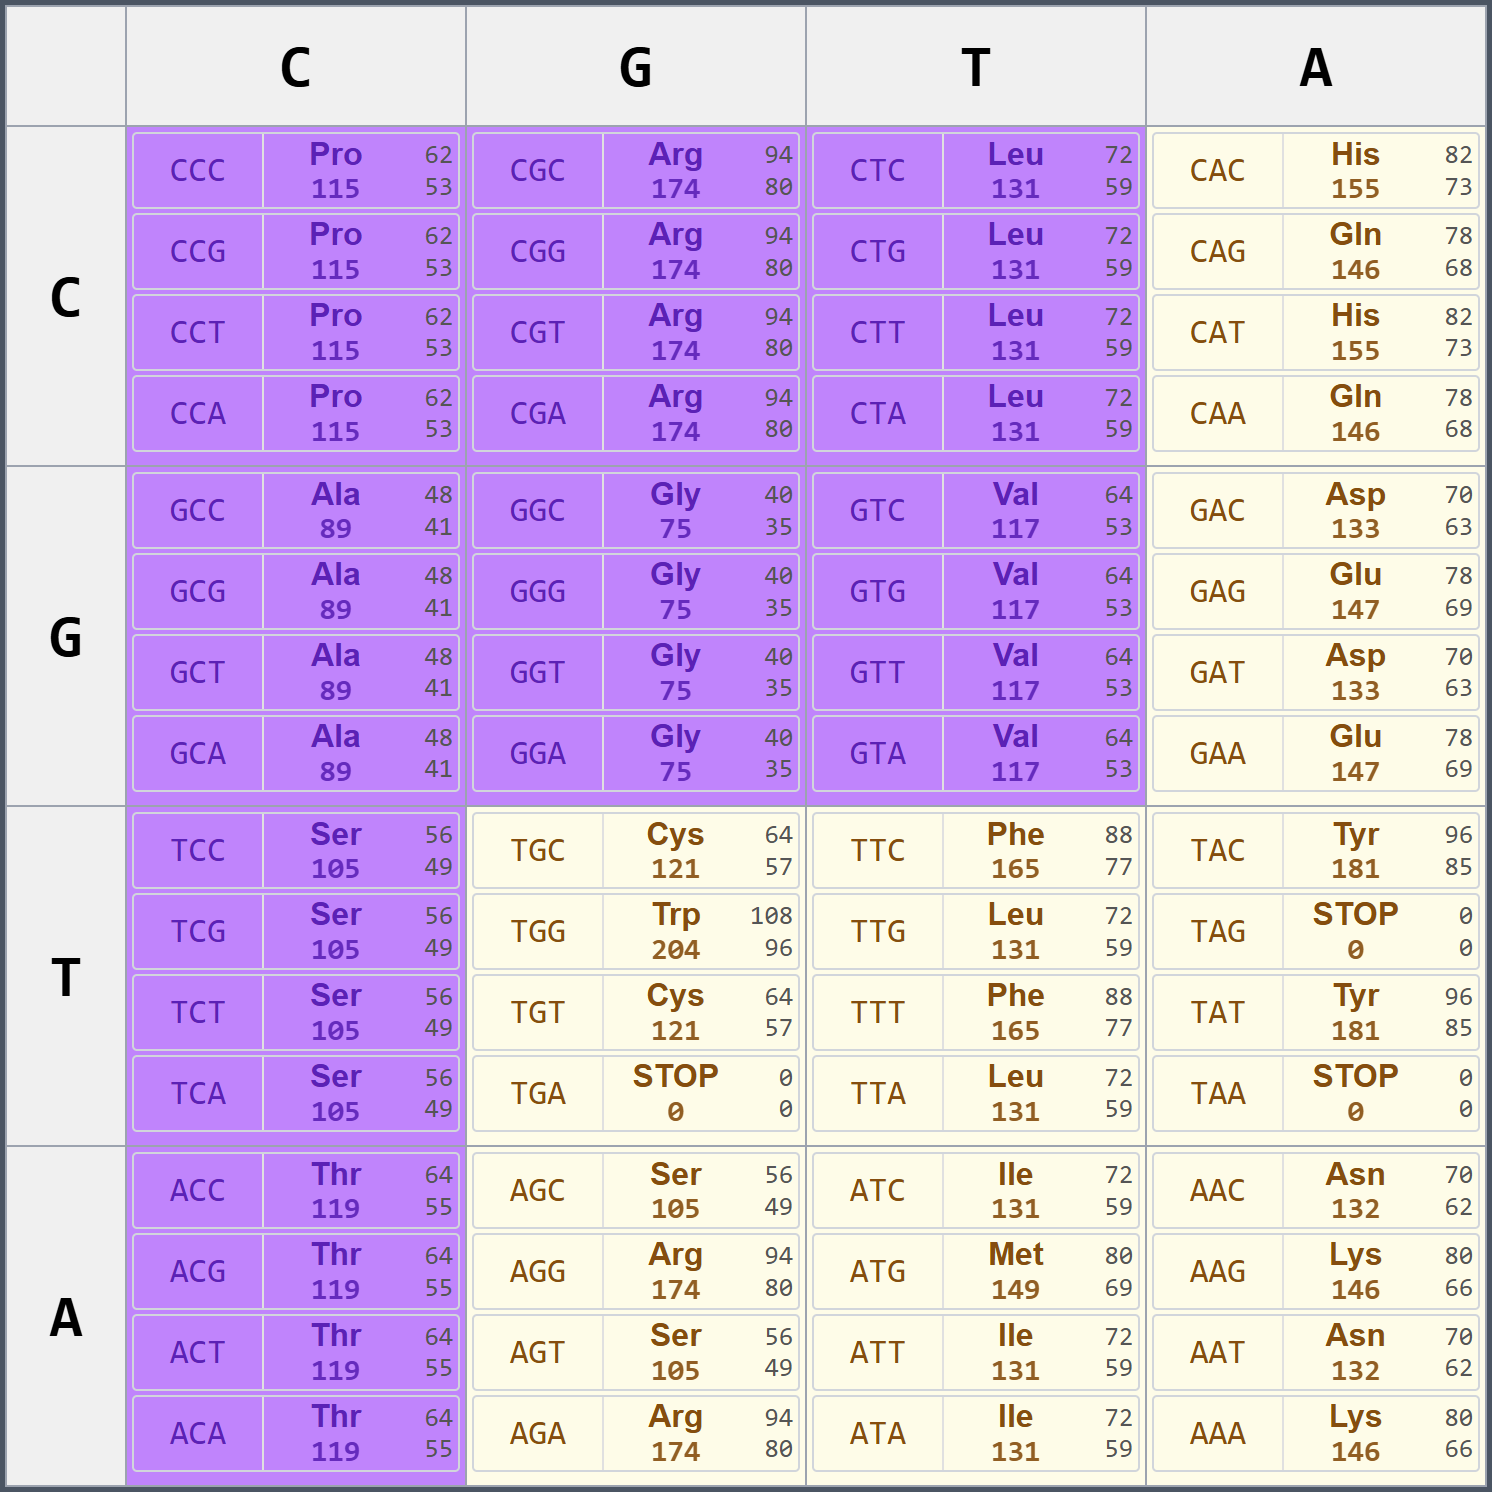
\includegraphics[width=0.85\textwidth]{codon_table_key0.png}
\caption{Standard genetic code with nucleon parameters of the encoded
amino acids, displayed under the naive reading (Key~0), in which stop
codons contribute zero and $\mathrm{ATG}$ is counted as methionine.
In each cell, the codon appears on the left; the symbol of the encoded
product (the three-letter amino acid symbol or $\mathrm{STOP}$ for
the three stop codons) appears at the top center; the total nucleon
count $T$ appears below the product symbol; the proton count $P$
appears at the top right; and the neutron count $N$ appears at the
bottom right. Codons of Octet~I (the eight fully
four-fold degenerate families) are shaded purple, and codons of
Octet~II are shaded yellow. Generated by the
accompanying \texttt{visualization.html}.}
  \label{fig:codon-table}
\end{figure}

\subsection{Codon-group construction}
\label{sec:partitioning}

In addition to the Rumer partition introduced in
Section~\ref{sec:genetic-code}, we use an additional overlapping
grouping system based on the chemical identity of the nucleotide at
the third codon position. Each of the four nucleotides belongs to
one of two classes under each of three distinct binary chemical
classifications:
\begin{itemize}
  \item base type: \emph{purine}
        $\{\mathrm{A},\mathrm{G}\}$ (R) or \emph{pyrimidine}
        $\{\mathrm{C},\mathrm{T}\}$ (Y);
  \item number of hydrogen bonds in the canonical base pair:
        \emph{strong} $\{\mathrm{C},\mathrm{G}\}$ (S; three bonds)
        or \emph{weak} $\{\mathrm{A},\mathrm{T}\}$ (W; two bonds);
  \item functional class: \emph{amino}
        $\{\mathrm{A},\mathrm{C}\}$ (M) or \emph{keto}
        $\{\mathrm{G},\mathrm{T}\}$ (K).
\end{itemize}
These axes were not selected in response to the subsequent
nucleon calculations: they are three conventional pairwise
dichotomies of the nucleotides and are represented explicitly
in the IUPAC--IUB ambiguity nomenclature by the symbol pairs
R/Y, S/W, and M/K. Together they exhaust the three
possible partitions of four nucleotides into two unordered
pairs, thereby yielding six two-element subsets
$X \subset \{\mathrm{A}, \mathrm{T}, \mathrm{G}, \mathrm{C}\}$.

For each of these six two-element subsets, and for each singleton
$X\in\{\{\mathrm{A}\},\{\mathrm{C}\},\{\mathrm{G}\},
\{\mathrm{T}\}\}$, we define the codon group
\[
G_X =
\{(c_1,c_2,c_3)\in\mathcal{C}_{64}
  : c_3\in X\}.
\]
Thus, $G_X$ consists of all codons whose third-position nucleotide
belongs to $X$. The six two-nucleotide groups overlap: every codon
belongs to exactly three of them, one for each chemical
classification. At the same time, every codon belongs to exactly
one of the four one-nucleotide groups.

This grouping system is applied at three levels: to all $64$
codons, to the $32$ codons of Octet~I, and to the $32$ codons of
Octet~II. If $|X|=2$, then $G_X$ contains $32$ codons, while each
of the intersections $G_X\cap\mathrm{Octet~I}$ and
$G_X\cap\mathrm{Octet~II}$ contains $16$ codons. If $|X|=1$, the
corresponding sizes are $16$ and $8$ codons. Group size alone does
not identify a particular group; formulas therefore specify the
set $X$ and, where necessary, the octet explicitly.

The family of $33$ codon groups used in the present work comprises
the full code as one group of $64$ codons; the two octets as groups
of $32$ codons each; ten groups $G_X$ at the full-code level,
corresponding to the six two-nucleotide and four one-nucleotide
sets $X$; and their twenty intersections with Octet~I and
Octet~II. Thus, the total number of analyzed groups is
\[
1+2+10+20=33.
\]
For example, $G_{\{\mathrm{G},\mathrm{T}\}}\cap
\mathrm{Octet~I}$ is the $16$-codon group
$\mathrm{Keto}\cap\mathrm{Octet~I}$, whereas
$G_{\{\mathrm{A}\}}\cap\mathrm{Octet~II}$ is the $8$-codon group
of Octet~II with adenine at the third position. All $33$ groups,
together with their sizes, codon compositions, and Rumer-octet
membership, are listed in the dataset \texttt{codon\_groups.csv}.

In the group registry, the full set $\mathcal{C}_{64}$ corresponds to
the row with id~1. In this article, that group is denoted
$\mathrm{All}$, whereas $\mathcal{C}_{64}$ denotes the codon set
itself.

\subsection{Pyrimidine synonymy and twin-group identities}
\label{sec:twin-identities}

Within every codon family of the standard genetic code, the codons
$\mathrm{NNC}$ and $\mathrm{NNT}$ with identical first two positions
encode the same amino acid. Therefore, exchanging
$\mathrm{C}\leftrightarrow\mathrm{T}$ at the third position does not
change the multiset of encoded amino acids. This exchange maps Keto
$\{\mathrm{G},\mathrm{T}\}$ to Strong
$\{\mathrm{C},\mathrm{G}\}$, and Amino
$\{\mathrm{A},\mathrm{C}\}$ to Weak
$\{\mathrm{A},\mathrm{T}\}$.

The two members of each pair contain the same service codons: Keto and
Strong contain $\mathrm{ATG}$ and $\mathrm{TAG}$, whereas Amino and
Weak contain $\mathrm{TAA}$ and $\mathrm{TGA}$. Therefore, under any
assignment $K$ that associates a pair of values $(P,N)$ with each
service codon (Section~\ref{sec:parametrization}) and for
$Q\in\{T,P,N,\Delta\}$, the identities
\[
Q_K(\mathrm{Keto})=Q_K(\mathrm{Strong}),\qquad
Q_K(\mathrm{Amino})=Q_K(\mathrm{Weak})
\]
hold. Intersecting both groups in either pair with the same octet
preserves these identities. The equalities are independent of
parametrization, although the full-group values themselves may depend
on~$K$. We refer to the Keto/Strong and Amino/Weak pairs, and to the
corresponding pairs formed by intersection with the same octet, as
\emph{twin groups}. In the dataset \texttt{codon\_groups.csv}, this
relationship is recorded in the \texttt{Twin\_Group\_ID} column.

Purine and Pyrimidine are not twin groups: exchanging
$\mathrm{C}\leftrightarrow\mathrm{T}$ preserves each of these groups
rather than mapping one to the other. The same pyrimidine synonymy
directly gives equality of all four nucleon quantities for the
one-nucleotide groups $\{\mathrm{C}\}$ and $\{\mathrm{T}\}$ and for
their intersections with either octet. These groups and their
intersections with the octets contain no service codons, so both the
values themselves and the equalities between them are independent of
parametrization. Because this is a pair of one-nucleotide groups rather
than a pair of two-nucleotide branches of the chemical axes, the term
\emph{twin groups} and the \texttt{Twin\_Group\_ID} column are not used
for it.

\subsection{Parametrization of service codons}
\label{sec:parametrization}

The nucleon quantities of a codon group are obtained by summing the
values of the amino acids encoded by its constituent codons in the
standard genetic code. For codons counted only according to their
amino-acid assignments, this summation is unambiguous. A separate
convention is needed for the three stop codons, which have no
amino-acid product, and for $\mathrm{ATG}$ in its initiator role;
$\mathrm{ATG}$ also encodes methionine
(Section~\ref{sec:genetic-code}).

The complete codon set $\mathcal{C}_{64}$, the four-codon service set
$\mathcal{S}$, and the remaining 60-codon pool
$\mathcal{C}_{\mathrm{SE}}$ are defined in
Section~\ref{sec:genetic-code}. We refer to
$\mathcal{C}_{\mathrm{SE}}$ below as the \emph{service-excluded pool};
its technical identifier in the code and file names is
\texttt{pool60}.
Every codon in $\mathcal{C}_{\mathrm{SE}}$ is unambiguously assigned
to a canonical amino acid. For
$c\in\mathcal{C}_{\mathrm{SE}}$ and
$Q\in\{T,P,N,\Delta\}$, $Q(c)$ denotes the corresponding quantity
of the free neutral form of the amino acid encoded by $c$, as defined
in Section~\ref{sec:composition}.

For any codon set $A\subseteq\mathcal{C}_{64}$ containing no service
codons, define
\[
Q(A):=\sum_{c\in A}Q(c).
\]
For a codon group $G$, its sum over the service-excluded pool is
defined by
\[
Q_{\mathrm{SE}}(G)
:=
\sum_{c\in G\cap\mathcal{C}_{\mathrm{SE}}}Q(c).
\]
For a service codon $c$, the notation $Q(c)$ without a key subscript
is not used because the formal contribution of such a codon depends
on the selected key. The
subscript $\mathrm{SE}$ indicates a restriction of the summation
domain, not a parametrization key. Neither the sum
$Q_{\mathrm{SE}}(G)$ nor the number of codons included in it,
$|G\cap\mathcal{C}_{\mathrm{SE}}|$, depends on the assignments to the
service codons.

If the group $G$ itself contains no service codons, the restriction
removes nothing and
\[
Q(G)=Q_{\mathrm{SE}}(G).
\]

To analyze the complete 64-position table, we introduce a
\emph{parametric key} $K$: a fixed assignment of a pair of numbers
$\bigl(P_K(c),N_K(c)\bigr)$ to every service codon $c$.
Under such a key, the group sums are defined by
\[
\bigl(P_K(G),N_K(G)\bigr)
:=
\bigl(P_{\mathrm{SE}}(G),N_{\mathrm{SE}}(G)\bigr)
+
\sum_{c\in G\cap\mathcal{S}}
\bigl(P_K(c),N_K(c)\bigr),
\]
and the remaining two quantities are derived rather than assigned
independently:
\[
T_K(G)=P_K(G)+N_K(G),
\qquad
\Delta_K(G)=P_K(G)-N_K(G).
\]
The same two relations define $T_K(c)$ and $\Delta_K(c)$ for each
service codon~$c$.
For $Q\in\{T,P,N,\Delta\}$, $Q_0(G)$ and $Q_1(G)$ below denote the
full group sums, including service-codon contributions, under the
Key~0 and Key~1 assignments, respectively. The subscripts $0$ and $1$
label these two assignments; they are not numerical values of a
scalar parameter. Thus $Q_{\mathrm{SE}}(G)$ is independent of the key,
whereas $Q_0(G)$ and $Q_1(G)$ can differ only through the
contributions of the service codons contained in group $G$. If group
$G$ contains no service codons, then
$Q_K(G)=Q(G)=Q_{\mathrm{SE}}(G)$ for every $K$. The subscript
$\mathrm{SE}$ applies only to codon groups; the subscripts $K$, $0$,
and $1$ apply to full group sums and to the formal contributions of
individual service codons. The two keys considered in this study are
recorded in \texttt{key\_parameters.csv}.

\paragraph{The naive reading (Key~0).}
Each of the three stop codons is assigned the zero contribution
$(P,N)=(0,0)$ because a termination signal has no amino acid product.
The $\mathrm{ATG}$ codon is treated as an ordinary methionine codon
and receives the values of the free methionine molecule,
$(P,N)=(80,69)$. This simple convention corresponds to the ordinary reading of the
amino-acid-coding part of the table, in which the stop signals are
assigned a zero contribution, but it remains a parametrization. In
particular, Key~0 is not identical to the service-excluded pool:
Key~0 retains all $64$ positions and counts $\mathrm{ATG}$ as
methionine, whereas in the pool the summation runs over the remaining
$60$ codons only.

\paragraph{Symmetrization (Key~1).}
Each of the three stop codons is assigned $(P,N)=(37,37)$, while
$\mathrm{ATG}$, treated as a formal initiation marker, is assigned
$(P,N)=(1,0)$. These values are not interpreted as the nucleon
composition of physical translation products. They are derived in
Sections~\ref{sec:results-key1-derivation}--%
\ref{sec:results-key1-uniqueness} under the assumption that the three
stop codons share a common parameter pair and under the conditions of
balance and divisibility by~$37$ specified there. Under these
assumptions, Key~1 is the unique minimal non-negative integer solution
of the resulting system. Minimality here means the smallest total contribution of
the service codons---the sum of the contributions of the
three stop codons and $\mathrm{ATG}$---determined
separately for protons and for neutrons. For the standard
code the balance fixes the difference between the stop and
start parameters, so the total contribution increases with
the start parameter and is minimal at its smallest
admissible value. Here Key~1 is introduced as the result
of that formal construction, not as a biochemical property of
termination signals or the initiator.

For codon groups containing no service codons, the values under
Key~0 and Key~1 coincide with the direct amino-acid sums. If a group
contains service codons, the Key~1 assignments have only a formal
arithmetic meaning: the corresponding sums do not represent the
nucleon composition of a physical ensemble of molecules. The terms
``proton count'', ``neutron count'' and ``total nucleon count'' are
retained for consistency with the underlying amino acid contributions,
but no biochemical interpretation is claimed for the formal Key~1
contributions.

The dataset \texttt{key\_parameters.csv} additionally contains eight
reference assignments, \texttt{Key~2}--\texttt{Key~9}, considered
during the exploratory stage. They are not used to obtain the results
of this study and do not have the status of the derived Key~1. The
following analysis therefore distinguishes three levels explicitly:
the service-excluded pool, the naive reading (Key~0), and the
symmetrization (Key~1).

\subsection{Analytical criteria and classification of equalities}
\label{sec:criteria}

For each of the $33$ codon groups defined in
Section~\ref{sec:partitioning}, we examine $P$, $N$, $T$, and
$\Delta$ at three analytical levels: the service-excluded pool,
Key~0, and Key~1. Three reporting procedures are described below:
tests of divisibility by~$37$ and
decimal roundness, and a search for exact equalities. Divisibility
by~$37$ is the primary preselected arithmetic criterion. Exact powers,
reduced ratios, and matches to amino acid differences are considered
separately as additional descriptive observations. Statistical
significance is assessed only where a corresponding null model is
specified.

\paragraph{Criterion 1: divisibility by 37.}
For every group quantity $P$, $N$, $T$ and $\Delta$, we compute the
quotient and remainder upon division by~$37$. A zero remainder denotes
exact divisibility. This criterion continues the line of investigation
opened by \citet{makukov2013} and developed by
\citet{panov2024}. When a value is divisible by~$37$, its displayed
factorization also exposes any further factors of the quotient; these
are not assigned separate evidential weight without an additional
analysis. Nonzero residues are reported descriptively only when they enter
exact relations among predefined groups or form recurring patterns of
one-unit deviations from the nearest multiple of~$37$.

Complete expressions of the form $q\cdot37+r$ for all groups and all
four quantities are provided in
\texttt{pool60\_divisibility-37.csv},
\texttt{key0\_divisibility-37.csv} and
\texttt{key1\_divisibility-37.csv}.

\paragraph{Criterion 2: roundness in the decimal system.}
We call a positive integer quantity round in the decimal system if it
is divisible by $10^k$ for at least one integer $k\geq1$; its degree
of roundness is the largest such $k$. This criterion is used
descriptively because the data contain exact multiples of $100$ and
$1000$, notably among the parametrization-independent Octet~I sums.
Although roundness is tied to decimal notation, the divisibility being
tested is a property of the integer itself: $10^k\mid x$ is equivalent
to simultaneous divisibility by $2^k$ and $5^k$. The systematic
control across prime moduli is presented in
Section~\ref{sec:discussion-controls}.

\paragraph{Criterion 3: exact equalities.}
At each analytical level, we compare the $P$, $N$, $T$, and $\Delta$
values of all $33$ groups and record every exact match. Trivial
identities such as $P(G)=P(G)$ are not included in the results. Each
equality is assigned to one of three classes:
\begin{itemize}
  \item \emph{different-size equalities}
        (\texttt{DIFF\_PARAM} in the \texttt{Match\_Type} column):
        the same numerical value is obtained by summing over different
        numbers of codons; either the same or different nucleon
        quantities may be compared;
  \item \emph{same-size cross-quantity equalities}
        (\texttt{CROSS\_PARAM}): the groups contain the same number of
        codons, but different quantities are compared, for example
        $P(G_1)=N(G_2)$;
  \item \emph{same-size same-quantity equalities}
        (\texttt{SAME\_PARAM}): the groups contain the same number of
        codons and the same quantity is compared, for example
        $P(G_1)=P(G_2)$.
\end{itemize}

For classification, group size is the number of codons actually
included in the sum. Under Key~0 and Key~1, this is the full size of
the group in the $64$-codon table. In the service-excluded pool, the
service codons are removed, so groups containing them are smaller.

All identified equalities are listed in
\texttt{pool60\_equalities.csv},
\texttt{key0\_equalities.csv} and
\texttt{key1\_equalities.csv}. Twin-group identities from
Section~\ref{sec:twin-identities} are also recorded, but are treated as
consequences of identical amino acid composition rather than as new
coincidences.

\paragraph{Additional exploratory observations.}
Beyond the primary procedures, we descriptively note:
\begin{itemize}
  \item exact powers of small integers, for example
        $4096=2^{12}$;
  \item reduced ratios within a group, including $P/T$, $N/T$,
        $\Delta/T$, $P/N$, $\Delta/P$ and $\Delta/N$, tabulated in
        \texttt{pool60\_ratios.csv},
        \texttt{key0\_ratios.csv} and
        \texttt{key1\_ratios.csv};
  \item matches between group-level quantities and the absolute
        differences $|\delta P|$, $|\delta N|$ or $|\delta T|$ of
        individual amino acid pairs, such as
        $|\delta N(\mathrm{Trp},\mathrm{Ile})|=37$.
\end{itemize}
These observations describe the arithmetic and may provide a basis
for testable hypotheses.

Finally, the four quantities are not independent:
\[
T=P+N,
\qquad
\Delta=P-N.
\]
Equalities, divisibility relations or ratios obtained from one another
through these identities are therefore not counted as separate
evidence. The same applies to copies propagated through nested groups
or twin-group identities. Section~\ref{sec:results} distinguishes
(i) facts computed directly for the service-excluded pool without
assigning values to the service codons; (ii) identities whose invariance to the
key is established algebraically; and (iii) results specific to
Key~0 or Key~1.

\subsection{Computed datasets and reproducibility}
\label{sec:datasets}

The principal deterministic results of this study are produced by
\texttt{reproduce.py}. The script reads five input datasets and
writes 17 computed output datasets. A separate deterministic script,
\texttt{controls.py}, writes four control datasets, whereas the
statistical analysis is performed by \texttt{mc\_significance.py},
which writes the summary table \texttt{mc\_significance.csv}, and is
independently re-checked by \texttt{verify\_mc.py}. By default, all
data paths are resolved relative to the directory of the corresponding
script.

\paragraph{Input datasets.}
Five input files define the numerical and structural basis of the
analysis:
\begin{itemize}
  \item \texttt{amino\_acids\_nucleons.csv} contains $P$, $N$, $T$
        and $\Delta$ for the twenty canonical amino acids
        (Section~\ref{sec:composition});
  \item \texttt{genetic\_code\_codons.csv} specifies the standard
        codon-to-translation-product mapping
        (Section~\ref{sec:genetic-code});
  \item \texttt{ncbi\_genetic\_code\_registry.csv} records a snapshot
        of the 27 NCBI translation tables, including the standard
        table (Section~\ref{sec:genetic-code});
  \item \texttt{codon\_groups.csv} defines the system of 33
        overlapping codon groups
        (Section~\ref{sec:partitioning});
  \item \texttt{key\_parameters.csv} contains the service-codon
        assignments of the parametric keys
        (Section~\ref{sec:parametrization}).
\end{itemize}

\paragraph{Per-key computed datasets.}
For each of the two principal keys, Key~0 and Key~1,
\texttt{reproduce.py} writes four files. The prefixes
\texttt{key0\_} and \texttt{key1\_} identify the active key:
\begin{itemize}
  \item \texttt{*\_nucleon-data.csv} contains the four reported
        group quantities $P$, $N$, $T$ and $\Delta$ for all 33
        groups; $T$ and $\Delta$ are derived from $P$ and $N$;
  \item \texttt{*\_divisibility-37.csv} expresses every quantity
        exactly as $q\cdot37+r$;
  \item \texttt{*\_equalities.csv} exhaustively enumerates exact
        numerical equalities and classifies them in the
        \texttt{Match\_Type} column as \texttt{DIFF\_PARAM},
        \texttt{CROSS\_PARAM} or \texttt{SAME\_PARAM}, following
        Section~\ref{sec:criteria};
  \item \texttt{*\_ratios.csv} contains the six ratios $P/T$, $N/T$,
        $\Delta/T$, $P/N$, $\Delta/P$ and $\Delta/N$ both as exact
        reduced fractions and as rounded decimal approximations.
\end{itemize}
The two keys therefore produce eight output files.

\paragraph{Service-excluded-pool datasets.}
For the service-excluded pool, the script writes four analogous
files:
\texttt{pool60\_nucleon-data.csv},
\texttt{pool60\_divisibility-37.csv},
\texttt{pool60\_equalities.csv} and
\texttt{pool60\_ratios.csv}. Before summation, the service codons are
removed from every group $G$, so that the number of codons included is
$|G\cap\mathcal{C}_{\mathrm{SE}}|$. No parametric key is applied.

\paragraph{Amino acid differences.}
Three files written once,
\texttt{amino\_acids\_proton\_differences.csv},
\texttt{amino\_acids\_neutron\_differences.csv} and
\texttt{amino\_acids\_nucleon\_differences.csv}, enumerate the
absolute differences $|\delta P|$, $|\delta N|$ and $|\delta T|$,
respectively, for all $\binom{20}{2}=190$ unordered pairs of
canonical amino acids.

\paragraph{Table-dependent NCBI pools.}
The remaining two outputs of the core script compare the standard
code with the other tables in
\texttt{ncbi\_genetic\_code\_registry.csv}. Because the sets of stop
codons differ between tables, we do not assume in advance that every
analyzed pool contains 60 codons. Two models are used. Model~1 excludes
$\mathrm{ATG}$ and every codon listed in the \texttt{Stop\_Codons}
field. Model~2 excludes $\mathrm{ATG}$ and only the permanent stop
codons marked \texttt{*} in the \texttt{Amino\_Acids} field;
context-dependent stops are included in the analysis with the amino
acid assignments recorded for them. The models coincide for tables
without context-dependent stops. For the standard table, both models
give the same 60-codon service-excluded pool. The actual number of
codons in the analyzed pool is recorded for both models (columns
\texttt{Pure\_Codons\_Count} and \texttt{Pure\_Codons\_Count\_Alt}).

\texttt{deficit\_models\_analysis.csv} contains one row for each of
the 27 tables. The full proton and neutron sums follow the registered
amino acid assignments, with positions marked
\texttt{*} contributing zero. For both models, the file additionally
records sums over the corresponding analyzed pool, the proton-sum
residue modulo~$37$, and three neutron deficits relative to:
\begin{enumerate}
  \item the constant $3700$ obtained for standard-code Octet~I;
  \item structural $T(\mathrm{Octet~I})$, retaining the eight
        families that occupy Octet~I positions in the standard table;
  \item functional $T(\mathrm{Octet~I})$, selecting in table $t$
        those four-codon families that have one amino acid assignment
        and no permanent stop codon.
\end{enumerate}

\texttt{keto\_amino\_balance\_models.csv} uses the same two models
and, for every table, sums $P$ and $N$ separately over the
intersections of the analyzed pool with the third-position Keto and
Amino groups. Both sums and the directed Keto-minus-Amino difference
are recorded.

\paragraph{Reproducibility of the core pipeline.}
\texttt{reproduce.py} uses only the Python standard library and
requires neither external packages nor a virtual environment. The
computation is deterministic: outputs are written in UTF-8 with LF
line endings and a fixed row order. The canonical repository files
are regenerated from the five inputs without manual editing. All
group sums and residues use integer arithmetic, while ratios are first
reduced exactly by their greatest common divisor. The decimal columns
in \texttt{*\_ratios.csv} are rounded representations of exact
fractions and are not used to obtain any result. Every deterministic
numerical claim can be traced to a specific cell or to a documented
exact combination of cells in the output files.

Neither \texttt{reproduce.py} nor \texttt{controls.py} uses
randomization. Randomization is confined to the separate Monte Carlo
analysis in \texttt{mc\_significance.py}, with a fixed seed and a
specified number of trials. Its tail-probability estimates and
uncertainty intervals necessarily use floating-point values.
\texttt{verify\_mc.py} independently re-implements the same analysis;
the statistical procedure is fully specified in
Section~\ref{sec:discussion-montecarlo}.

\paragraph{Supplementary visualizer.}
\texttt{visualization.html} provides an interactive view of the
translation tables and codon groups under the service-excluded pool
(POOL60), Key~0 and Key~1, together with additional exploratory
views. It is not part of the core reproducible pipeline and is not
the source of published numerical results: values reported in the
main text are checked against the deterministic CSV files. An online
version is available at
\url{https://ruslankhafizov.github.io/genetic-code-arithmetic/}.

\paragraph{Supplementary control datasets.}
\texttt{controls.py} reads the same five input files, uses only the
Python standard library and writes four deterministic datasets:
\begin{itemize}
  \item \texttt{position\_axis\_analysis.csv} separately applies
        the three binary chemical classifications Keto/Amino,
        Strong/Weak and Purine/Pyrimidine to the first, second and
        third codon positions at three analytical levels:
        the service-excluded pool, Key~0 and Key~1. For each side it
        records the four nucleon quantities and their residues
        modulo~$37$;
  \item \texttt{prime\_divisibility\_scan.csv} scans every prime up
        to~$97$ over three value sets: group quantities identical under
        Key~0 and Key~1, all Key~0 quantities, and all Key~1
        quantities. For each prime it records the numbers of
        divisible instances, distinct nonzero values and distinct odd
        cores, together with a reference value $n/p$ for $n$ distinct
        values. This reference describes residue uniformity and is not
        a statistical null model or a $p$-value;
  \item \texttt{position\_asymmetry\_ncbi.csv} applies the
        Keto/Amino classification to each of the three positions of
        all 27 NCBI tables under Model~1 and Model~2. For $T$,
        $P$, $N$ and
        $\Delta$, it records directed Keto-minus-Amino differences,
        their residues modulo~$37$ and position-level summary flags;
  \item \texttt{representation\_sensitivity.csv} recomputes 13
        explicitly listed absolute and difference quantities under
        three representations of the encoded amino acid. Relative to
        the neutral free molecule, the proton and neutron offsets are
        $(0,0)$ for the free molecule itself, $(-10,-8)$ for the
        peptide residue, and $(0,0)$ for the zwitterion. For every
        quantity, the file records the result under each representation
        and its agreement with the free-molecule baseline.
\end{itemize}
These four files define the positional, modular, cross-table and
representation-specificity controls. Their results are interpreted
in Section~\ref{sec:discussion-controls}.

\paragraph{Data and code availability.}
The accompanying repository contains the manuscript sources, five
input datasets, 17 core computed datasets, four control datasets, the
Monte Carlo summary table \texttt{mc\_significance.csv}, four Python
scripts and the interactive visualizer. Complete run commands and
descriptions of the dataset columns are provided in the repository
README:
\url{https://github.com/RuslanKhafizov/genetic-code-arithmetic}.
Versions of the materials are archived at Zenodo under the concept
DOI
\href{https://doi.org/10.5281/zenodo.20360037}
     {10.5281/zenodo.20360037}.

\section{Results}
\label{sec:results}

The arithmetic properties are considered here at three analytical
levels. The first level (Section~\ref{sec:results-independent})
comprises facts established without assigning values to the service
codons.

The second level (Section~\ref{sec:results-key0}) is the naive reading
(Key~0), in which the three stop codons are assigned a contribution of
zero and the initiator $\mathrm{ATG}$ is counted as methionine.

Section~\ref{sec:results-localization} reduces the asymmetry of the
Keto and Amino branches to the nucleon differences of the
$\mathrm{Trp}$--$\mathrm{Ile}$ pair and examines the parity constraint
on the proton quantities.

At the third level, Section~\ref{sec:results-key1-derivation}
derives Key~1, the unique minimal non-negative integer assignment to
the service codons determined by the joint conditions of nucleon-pool
balance along the Keto/Amino axis and divisibility of the global pools
by~$37$; equivalently, this balance augments the
$\mathrm{C}/\mathrm{T}$ symmetry imposed by the code with
$\mathrm{G}/\mathrm{A}$ symmetry in proton and neutron sums grouped by
the nucleotide in the third position.

Section~\ref{sec:results-key1-consequences} uses this formal assignment
to extend the arithmetic analysis to the complete $64$-codon table and
distinguishes between identities that follow directly from the
derivation conditions and additional regularities not used to select
Key~1.

Section~\ref{sec:results-synthesis} draws together the findings of all
three levels.

The standard code remains the principal object of analysis
throughout. Alternative NCBI translation tables are examined later
for comparison and to assess the specificity of the results.

\subsection{Parametrization-independent results}
\label{sec:results-independent}

The parametrization-independent results for group-level nucleon
quantities in this subsection are obtained under one of two conditions:
either the summation domain is restricted to the service-excluded pool,
or the group under consideration itself contains no service codons.

These results form the basis of the arithmetic structure that is
traced further as the service codons are restored. The neutron sum of the service-excluded pool is divisible by~$37$,
whereas the proton sum falls one unit short of the nearest multiple.
Through the difference~$\Delta$ this deviation is traced to the codons
with $\mathrm{G}$ at the third position within Octet~II~--- the group
that contains the initiator $\mathrm{ATG}$ in the full table
(Section~\ref{sec:results-sensepool}). The nucleon sum of Octet~I is
divisible by~$37$, and all four of its quantities are divisible
by~$100$ (Section~\ref{sec:results-octetI}). For the
pyrimidine-restricted groups of the full code the difference~$\Delta$
lies on the lattice of step~$37$, whereas the deviations arising on
intersection with the octets cancel within the group
(Section~\ref{sec:results-pyrimidine}).

\subsubsection{The service-excluded pool}
\label{sec:results-sensepool}

The Keto/Amino and Strong/Weak partitions of $\mathcal{C}_{\mathrm{SE}}$
give pairwise equal neutron and proton sums, owing to pyrimidine synonymy
(Section~\ref{sec:twin-identities}):
\[
\begin{aligned}
N_{\mathrm{SE}}(\mathrm{Keto}) = N_{\mathrm{SE}}(\mathrm{Strong})
  &= 1813 = 49 \cdot 37, \\
N_{\mathrm{SE}}(\mathrm{Amino}) = N_{\mathrm{SE}}(\mathrm{Weak})
  &= 1776 = 48 \cdot 37, \\
P_{\mathrm{SE}}(\mathrm{Keto}) = P_{\mathrm{SE}}(\mathrm{Strong})
  &= 2108 = 57 \cdot 37 - 1, \\
P_{\mathrm{SE}}(\mathrm{Amino}) = P_{\mathrm{SE}}(\mathrm{Weak})
  &= 2072 = 56 \cdot 37.
\end{aligned}
\]
Both neutron sums lie on the $37$-lattice separately. The proton sum of
the Amino half lands on it exactly, whereas the Keto half falls one unit
short of the nearest multiple. Adding the halves gives, for the pool as a
whole,
\[
N(\mathcal{C}_{\mathrm{SE}}) = 3589 = 97 \cdot 37,
\qquad
P(\mathcal{C}_{\mathrm{SE}}) = 4180 = 113 \cdot 37 - 1,
\qquad
\Delta(\mathcal{C}_{\mathrm{SE}}) = 591 = 16 \cdot 37 - 1.
\]

Analysis of $\Delta$ localizes the one-unit deviation of the proton sum
of the pool from the nearest multiple of~$37$ in the group $\{\mathrm{G}\}
\cap \mathrm{Octet~II}$. On the Keto/Amino and Strong/Weak axes the
neutron sums are multiples of~$37$, so $\Delta = P - N$ has the same
residue as the proton sum. On the Purine/Pyrimidine axis neither $P$ nor
$N$ lies on the lattice, but their residues coincide for Pyrimidine and
differ by one for Purine:
\[
\begin{aligned}
\Delta_{\mathrm{SE}}(\mathrm{Keto}) = \Delta_{\mathrm{SE}}(\mathrm{Strong})
  = \Delta_{\mathrm{SE}}(\mathrm{Purine})
  &= 295 = 8 \cdot 37 - 1, \\
\Delta_{\mathrm{SE}}(\mathrm{Amino}) = \Delta_{\mathrm{SE}}(\mathrm{Weak})
  = \Delta(\mathrm{Pyrimidine})
  &= 296 = 8 \cdot 37.
\end{aligned}
\]

Keto, Strong, Amino, and Weak each contain $30$ codons in the pool, Purine
contains $28$, and Pyrimidine contains $32$. The same two values of
$\Delta$, $295$ and $296$, arise in all three partitions --- both for
parts of equal size $30/30$ and for the unequal split $28/32$.

At the level of the one-nucleotide groups none of the sums $P$ and $N$ is
a multiple of~$37$, and the one-unit deviation in~$\Delta$ is carried by one group
--- the branch $\{\mathrm{G}\}$, common to Keto, Strong, and Purine:
\[
\Delta_{\mathrm{SE}}(\{\mathrm{G}\}) = 147 = 4 \cdot 37 - 1,
\qquad
\Delta_{\mathrm{SE}}(\{\mathrm{A}\}) =
\Delta(\{\mathrm{C}\}) =
\Delta(\{\mathrm{T}\}) = 148 = 4 \cdot 37.
\]
Keto, Strong, and Purine are the unions of $\{\mathrm{G}\}$ with
$\{\mathrm{T}\}$, $\{\mathrm{C}\}$, and $\{\mathrm{A}\}$ respectively. The
one-unit deviation localized in $\Delta_{\mathrm{SE}}(\{\mathrm{G}\})$
can therefore be traced across all three axes.

Within Octet~I all four one-nucleotide groups have $\Delta = 75$, so
the difference falls entirely in Octet~II:
\[
\Delta_{\mathrm{SE}}(\{\mathrm{G}\} \cap \mathrm{Octet~II}) = 72,
\qquad
\Delta_{\mathrm{SE}}(\{\mathrm{A}\} \cap \mathrm{Octet~II}) =
\Delta(\{\mathrm{C}\} \cap \mathrm{Octet~II}) =
\Delta(\{\mathrm{T}\} \cap \mathrm{Octet~II}) = 73.
\]
In the pool the groups $\{\mathrm{G}\} \cap \mathrm{Octet~II}$ and
$\{\mathrm{A}\} \cap \mathrm{Octet~II}$ contain six codons each, whereas
$\{\mathrm{C}\} \cap \mathrm{Octet~II}$ and $\{\mathrm{T}\} \cap
\mathrm{Octet~II}$ contain eight. The observed distribution of the values
$72$ and $73$ therefore cannot be attributed to group size.

On passing to the complete $64$-codon table, these two six-codon branches
are supplemented by different pairs of service codons: $\{\mathrm{A}\}
\cap \mathrm{Octet~II}$ by the stop codons $\mathrm{TAA}$ and
$\mathrm{TGA}$, and $\{\mathrm{G}\} \cap \mathrm{Octet~II}$ by the stop
codon $\mathrm{TAG}$ and the initiator $\mathrm{ATG}$. As will be shown in
the derivation of Key~1 (Section~\ref{sec:results-key1-derivation}), the
formal $\Delta$-contribution under that assignment equals~$1$ for the
initiator $\mathrm{ATG}$ and~$0$ for each stop codon. Therefore, under
Key~1,
\[
\Delta_{1}(\{\mathrm{G}\} \cap \mathrm{Octet~II})
  = 72 + 1 + 0 = 73,
\qquad
\Delta_{1}(\{\mathrm{A}\} \cap \mathrm{Octet~II})
  = 73 + 0 + 0 = 73.
\]
The missing unit is thus returned through the initiator $\mathrm{ATG}$,
aligning the two branches. Since $\mathrm{ATG}$ belongs to the branch
$\{\mathrm{G}\}$ and to Keto, Strong, and Purine, the same single
contribution simultaneously compensates for the deviation in all of these
groups and in the value of $\Delta$ for the complete table under Key~1.

The full hierarchy of groups for the service-excluded pool, together with
the corresponding nucleon quantities, is shown in Figure~\ref{fig:pool60}.

\begin{figure}[p]
\centering
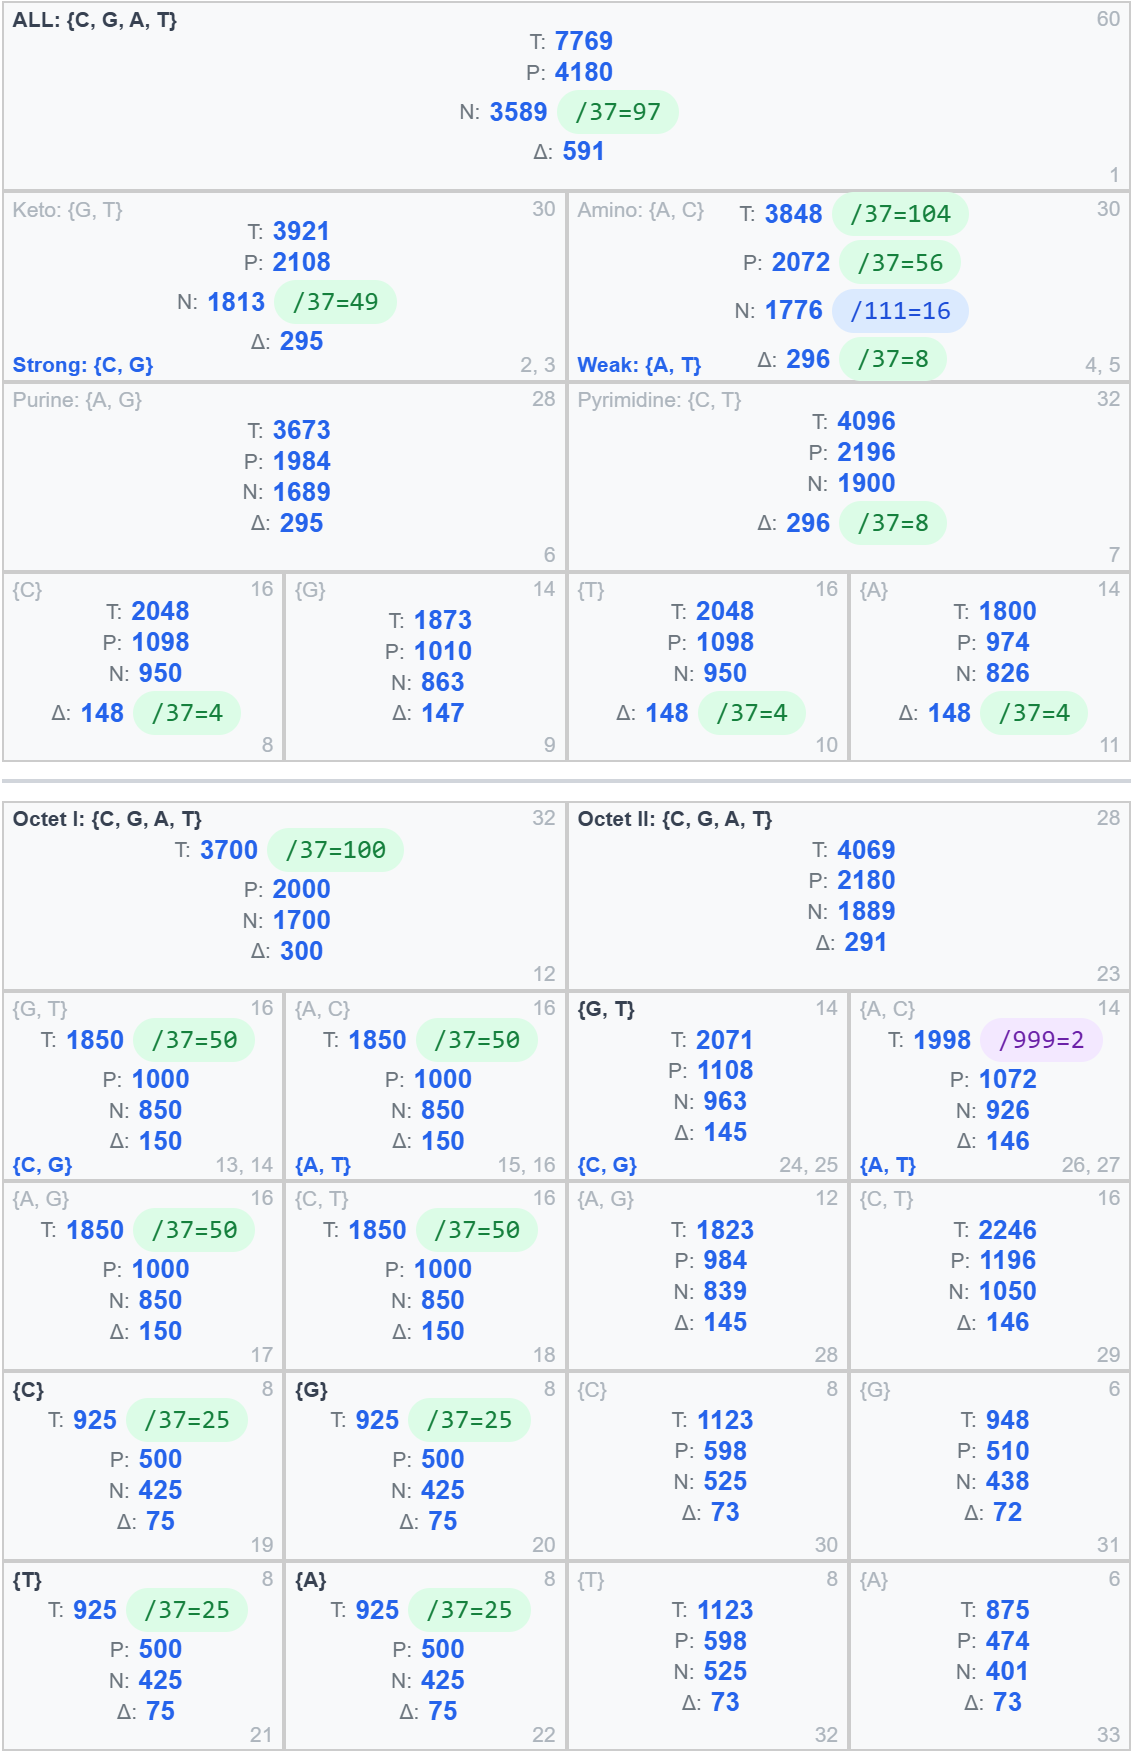
\includegraphics[width=0.72\textwidth]{pool60_structure.png}
\caption{Structure of the service-codon-excluded 60-codon pool
$\mathcal{C}_{\mathrm{SE}}$ (\texttt{pool60}). For each group, all four
quantities are computed using only the non-service codons it contains; the
three stop codons and the initiator $\mathrm{ATG}$ are excluded, so every
quantity shown is independent of parametrization. The quantities shown are
the total
nucleon sum~$T$, proton sum~$P$, neutron sum~$N$,
and hydrogen atom count $\Delta = P - N$. Cell layout: the group name
appears in the upper-left corner, the number of codons remaining in the
group in the upper-right corner, and the identifier from
\texttt{codon\_groups.csv} in the lower-right corner; twin pairs of groups
with identical values are collapsed into a single cell, with the second
name in the lower-left corner and both identifiers listed, separated by a
comma, in the lower-right corner. Green, blue, and purple highlights
indicate divisibility by~$37$, $111 = 3 \cdot 37$, and $999 = 27 \cdot
37$, respectively; the largest applicable modulus is marked.
Figures~\ref{fig:groups-key0} and~\ref{fig:groups-key1} use the same grid
and color code, but represent the complete $64$-codon table. All three
figures were generated by the \texttt{visualization.html} script.}
\label{fig:pool60}
\end{figure}

\subsubsection{Arithmetic of Octet~I}
\label{sec:results-octetI}

Octet~I (id~12) contains no service codons, so its nucleon quantities
are independent of any parametrization:
\[
\begin{aligned}
T(\mathrm{Octet~I}) &= 3700 = 100 \cdot 37, &
P(\mathrm{Octet~I}) &= 2000 = 2 \cdot 1000, \\
N(\mathrm{Octet~I}) &= 1700 = 17 \cdot 100, &
\Delta(\mathrm{Octet~I}) &= 300 = 3 \cdot 100.
\end{aligned}
\]
All four quantities are multiples of~$100$, while the proton sum
$P(\mathrm{Octet~I})$ is also a multiple of~$1000$. In addition, the
nucleon sum $T(\mathrm{Octet~I})$ is divisible by~$37$.

Octet~I consists of eight fully four-fold degenerate codon families.
Each of its six $16$-codon groups (ids~13--18) contains two codons from
every family, so each of its nucleon quantities equals half the
corresponding quantity of the whole octet:
\[
T = 1850 = 50 \cdot 37, \qquad
P = 1000 = 10^{3}, \qquad
N = 850, \qquad
\Delta = 150.
\]
Each of its four $8$-codon groups (ids~19--22) contains one codon from
every family, so its quantities equal one quarter of the whole-octet
values:
\[
T = 925 = 25 \cdot 37, \qquad
P = 500 = 5 \cdot 100, \qquad
N = 425, \qquad
\Delta = 75 = 2 \cdot 37 + 1.
\]
Thus, at all three levels of the Octet~I hierarchy, exact scaling
preserves divisibility of the nucleon sum $T$ by~$37$ and a single
rational profile with a common denominator of~$37$:
\[
\frac{P}{T} = \frac{20}{37},
\qquad
\frac{N}{T} = \frac{17}{37},
\qquad
\frac{\Delta}{T} = \frac{3}{37}.
\]

The proton and neutron sums of the whole octet have residues $+2$ and
$-2$ modulo~$37$, which cancel in $T = P + N$. The neutron residue
$-2$ of Octet~I is, in turn, compensated by the residue $+2$ of the
Octet~II neutron sum in the service-excluded pool. Adding the neutron
sums of the two octets gives the pool neutron sum
$N(\mathcal{C}_{\mathrm{SE}})$ obtained in
Section~\ref{sec:results-sensepool}. Both cancellations are represented
by the following equalities:
\[
\begin{aligned}
P(\mathrm{Octet~I})
  &= 2000 = 54 \cdot 37 + 2, \\
N(\mathrm{Octet~I})
  &= 1700 = 46 \cdot 37 - 2, \\
N_{\mathrm{SE}}(\mathrm{Octet~II})
  &= 1889 = 51 \cdot 37 + 2, \\
N(\mathcal{C}_{\mathrm{SE}})
  &= N(\mathrm{Octet~I})
   + N_{\mathrm{SE}}(\mathrm{Octet~II}) \\
  &= 1700 + 1889 = 3589 = 97 \cdot 37.
\end{aligned}
\]

At the $16$-codon level, exact halving gives residues $+1$ for $P$ and
$-1$ for $N$ modulo~$37$.
Of the four $8$-codon groups, the two pyrimidine groups---
$\{\mathrm{C}\} \cap \mathrm{Octet~I}$ (id~19) and
$\{\mathrm{T}\} \cap \mathrm{Octet~I}$ (id~21)---form the Pyrimidine
group within Octet~I (id~18), which enters the pyrimidine cascade in
Section~\ref{sec:results-pyrimidine}.

\subsubsection{Arithmetic of pyrimidine-restricted groups}
\label{sec:results-pyrimidine}

By pyrimidine synonymy (Section~\ref{sec:twin-identities}), the
$\{\mathrm{C}\}$ and $\{\mathrm{T}\}$ groups have identical nucleon
quantities at the full-code level and after intersection with either
octet. Together they form the Pyrimidine group (id~7). These groups and
their octet intersections contain no service codons, so their values
are independent of parametrization. Unlike the Octet~I hierarchy, the
full Pyrimidine group spans both octets and includes partially
degenerate codon families. Therefore, not all values at its lower
levels are obtained by a single exact scaling; they are examined
separately below.

For the full Pyrimidine group, the nucleon quantities are
\[
\begin{aligned}
T(\mathrm{Pyrimidine}) &= 4096 = 2^{12}, &
P(\mathrm{Pyrimidine}) &= 2196, \\
N(\mathrm{Pyrimidine}) &= 1900 = 19 \cdot 100, &
\Delta(\mathrm{Pyrimidine}) &= 296 = 8 \cdot 37.
\end{aligned}
\]
Here, $\Delta$ satisfies the primary preselected criterion of
divisibility by~$37$, and $N = 1900$ satisfies the roundness criterion.
The exact power of two $T = 2^{12}$ is an additional descriptive
observation.

By the C/T identity, the two $16$-codon groups $\{\mathrm{C}\}$
(id~8) and $\{\mathrm{T}\}$ (id~10) have identical nucleon
quantities. Because they partition the Pyrimidine group, each value is
half the corresponding full-group value:
\[
\begin{aligned}
T(\{\mathrm{C}\}) = T(\{\mathrm{T}\})
  &= 2048 = 2^{11}, &
P(\{\mathrm{C}\}) = P(\{\mathrm{T}\})
  &= 1098, \\
N(\{\mathrm{C}\}) = N(\{\mathrm{T}\})
  &= 950, &
\Delta(\{\mathrm{C}\}) = \Delta(\{\mathrm{T}\})
  &= 148 = 4 \cdot 37.
\end{aligned}
\]
The entire profile at this level is therefore obtained by exact scaling
and does not form a separate set of independent regularities.

At the $8$-codon level, all four Octet~I groups, including
$\{\mathrm{C}\} \cap \mathrm{Octet~I}$ (id~19) and
$\{\mathrm{T}\} \cap \mathrm{Octet~I}$ (id~21), have
$\Delta = 75$ (Section~\ref{sec:results-octetI}). The corresponding
$\{\mathrm{C}\} \cap \mathrm{Octet~II}$ (id~30) and
$\{\mathrm{T}\} \cap \mathrm{Octet~II}$ (id~32) groups have
$\Delta = 73$. Their unions within the octets form the
$\mathrm{Pyrimidine} \cap \mathrm{Octet~I}$ (id~18) and
$\mathrm{Pyrimidine} \cap \mathrm{Octet~II}$ (id~29) groups. These
values form the following cascade:
\[
\begin{aligned}
\Delta(\{\mathrm{C}\} \cap \mathrm{Octet~I})
  = \Delta(\{\mathrm{T}\} \cap \mathrm{Octet~I})
  &= 75 = 2 \cdot 37 + 1, \\
\Delta(\{\mathrm{C}\} \cap \mathrm{Octet~II})
  = \Delta(\{\mathrm{T}\} \cap \mathrm{Octet~II})
  &= 73 = 2 \cdot 37 - 1, \\
\Delta(\mathrm{Pyrimidine} \cap \mathrm{Octet~I})
  &= 2 \cdot 75 = 150 = 4 \cdot 37 + 2, \\
\Delta(\mathrm{Pyrimidine} \cap \mathrm{Octet~II})
  &= 2 \cdot 73 = 146 = 4 \cdot 37 - 2, \\
\Delta(\mathrm{Pyrimidine})
  &= 150 + 146 = 296 = 8 \cdot 37.
\end{aligned}
\]
The one-unit deviations of opposite sign, $+1$ and $-1$, double to
$+2$ and $-2$ when the groups within each octet are added, and cancel
when the octets are added. Thus, the values $150$, $146$, and $296$
belong to one additive scheme rather than constituting independent
results.

The relation of the pyrimidine cascade to the pattern of one-unit
deviations in the proton and neutron sums is considered under Key~0
(Section~\ref{sec:results-key0-delta}).

The pyrimidine cascade should also be distinguished from the one-unit
deviation of $\Delta_{\mathrm{SE}}(\{\mathrm{G}\})$ from the lattice
of step~$37$ (Section~\ref{sec:results-sensepool}). The pyrimidine
deviations cancel between the octets, whereas the deviation of the
$\{\mathrm{G}\}$ group is not compensated when it is combined with
another one-nucleotide group and propagates to the Keto, Strong, and
Purine groups. Because the neutron sums of Keto and Strong in the
service-excluded pool are multiples of~$37$, the identity
$P=N+\Delta$ implies that their proton sums have the same one-unit
deviation, $-1$.

\subsection{Results under Key~0}
\label{sec:results-key0}

Under the naive reading (Key~0), summation is performed over the complete
$64$-codon table: the stop-codon contribution is zero, whereas the initiator
$\mathrm{ATG}$ is counted as methionine
(Section~\ref{sec:parametrization}). Thus, in passing from the
service-excluded pool to the complete table, the only nonzero contribution
comes from $\mathrm{ATG}$:
\[
\bigl(T(\mathrm{Met}),P(\mathrm{Met}),N(\mathrm{Met}),
\Delta(\mathrm{Met})\bigr)=(149,80,69,11).
\]

The deviations from the nearest multiples of~$37$ for the service-excluded
pool, methionine, and the complete $64$-codon table are related as
\[
(-1,-1,0,-1)+(+1,+6,-5,+11)=(0,+5,-5,+10).
\]
The $\mathrm{ATG}$ contribution brings the nucleon sum $T$ exactly onto the
$37$-lattice, since $149=4\cdot37+1$ exactly compensates the one-unit
deviation $-1$, but at the same time moves the neutron sum off the lattice,
although it is divisible by~$37$ in the pool
(Section~\ref{sec:results-sensepool}).

Below, we show how this transformation propagates through the nested
groups containing $\mathrm{ATG}$. In the Amino and Weak groups, all
the restored positions are occupied by stop codons, so the sums of the
complete $32$-codon groups coincide numerically with the sums over the
$30$ codons in the corresponding branches of the service-excluded
pool. These sums already lie on the $37$-lattice
(Section~\ref{sec:results-sensepool}), and the divisibility is
therefore preserved in passing to the complete table. Under Key~0,
restoring the service positions makes the groups on the two sides of
the mirror pattern of one-unit deviations equal in size. The pattern
appears at two levels: at the $16$-codon level in the proton and
neutron sums, and at the $8$-codon level in the difference $\Delta$.
Within Octet~II at the $8$-codon level, this pattern, established
earlier for the pyrimidine groups
(Section~\ref{sec:results-pyrimidine}), also extends to the
$\{\mathrm{A}\}$ group: its value of $\Delta$ already coincided with
theirs in the pool, while restoring the service positions makes all
three groups equal in size. The sole
exception is the $\{\mathrm{G}\}$ branch, which contains
$\mathrm{ATG}$.

The overall pattern of group quantities under Key~0 is shown in
Fig.~\ref{fig:groups-key0}.

\begin{figure}[!htbp]
  \centering
  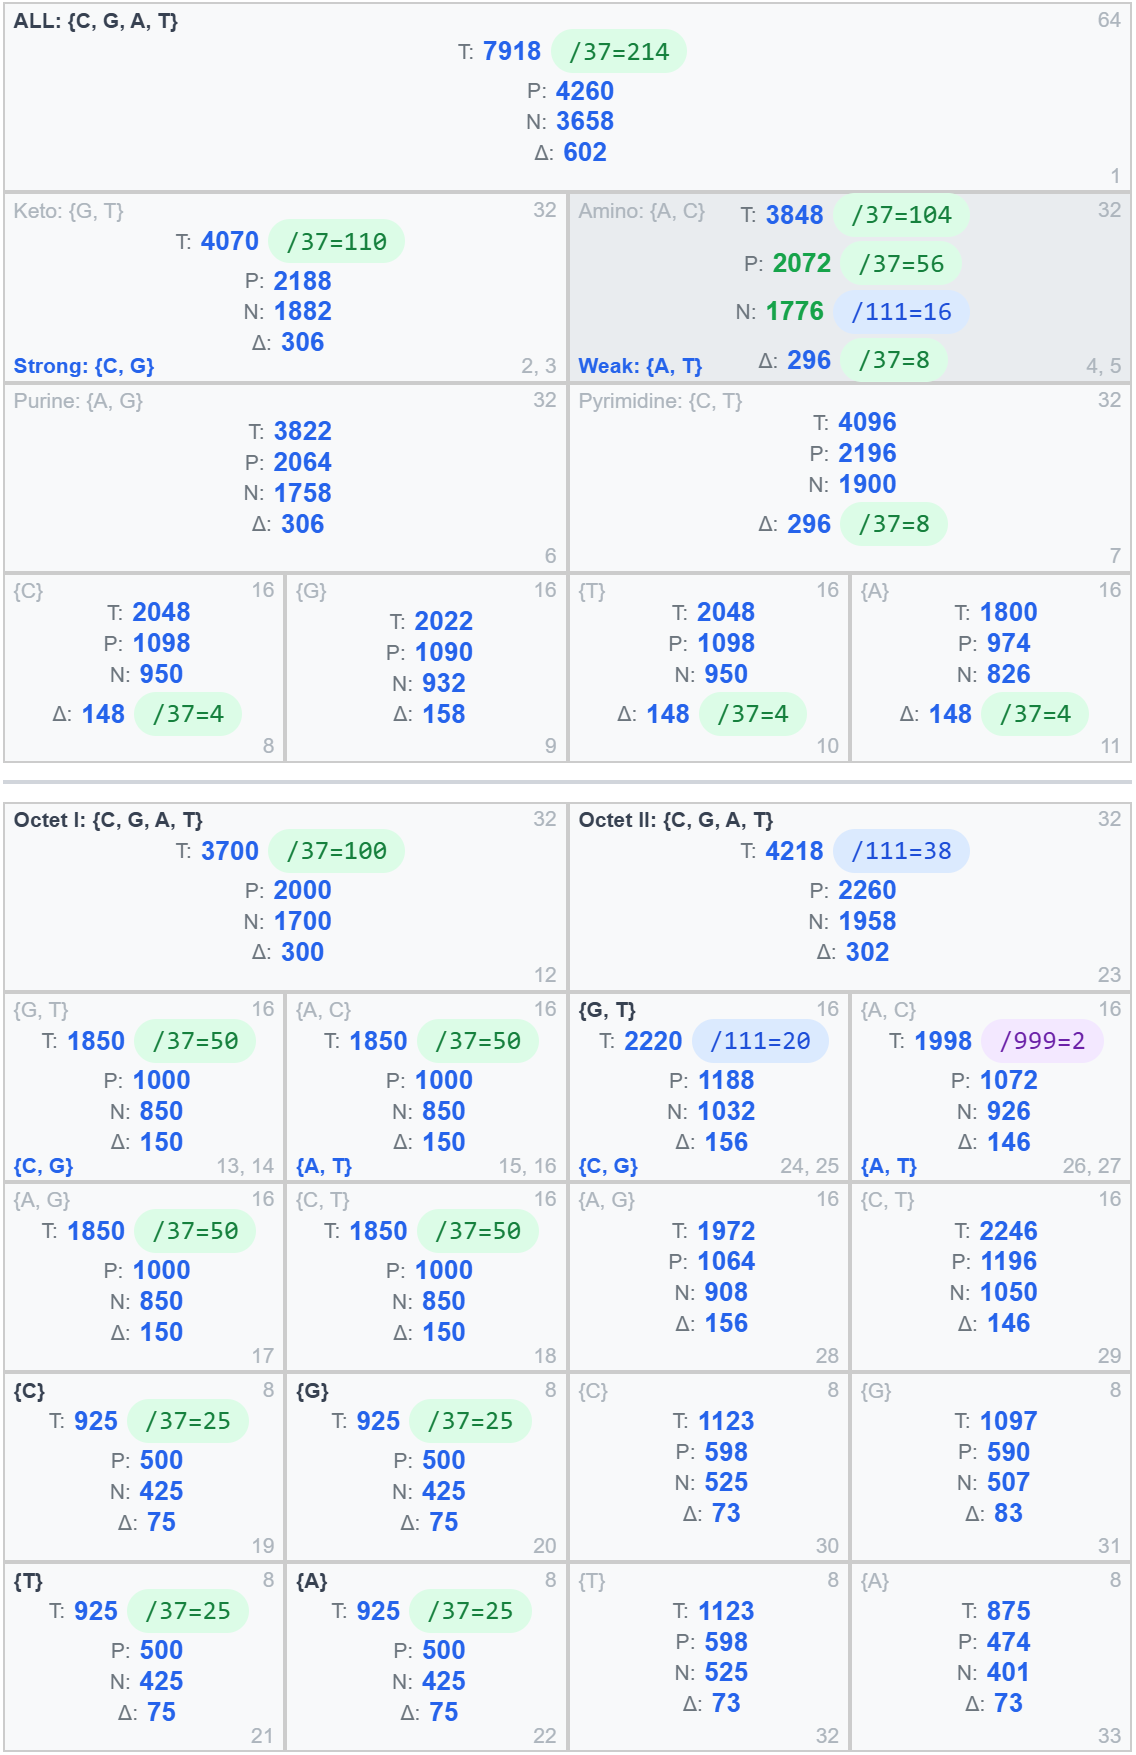
\includegraphics[width=0.78\textwidth]{groups_key0.png}
  \caption{Nucleon quantities $T$, $P$, $N$, and $\Delta$ for all
  codon groups under Key~0. The grid, twin-group pair merging, and
  divisibility color code are the same as in
  Fig.~\ref{fig:pool60}, but the quantities are calculated for the
  complete $64$-codon table. Generated with
  \texttt{visualization.html}.}
  \label{fig:groups-key0}
\end{figure}

\subsubsection{Divisibility of \texorpdfstring{$T$}{T} by
\texorpdfstring{$37$}{37} at the upper levels of partitioning}

The $\mathrm{ATG}$ contribution falls in Octet~II. Under Key~0, its
four $8$-codon groups have the following profile:
\[
\begin{aligned}
T(\{\mathrm{C}\}\cap\mathrm{Octet~II})
  =T(\{\mathrm{T}\}\cap\mathrm{Octet~II})
  &=1123=30\cdot37+13, \\
T_{0}(\{\mathrm{A}\}\cap\mathrm{Octet~II})
  &=875=24\cdot37-13, \\
T_{0}(\{\mathrm{G}\}\cap\mathrm{Octet~II})
  &=1097=30\cdot37-13.
\end{aligned}
\]
The pyrimidine branches deviate from the nearest multiple by $+13$,
the purine branches by $-13$. In the service-excluded pool, the
deviation of the $\{\mathrm{G}\}$ branch differs by one unit from
that of the $\{\mathrm{A}\}$ branch:
\[
T_{\mathrm{SE}}(\{\mathrm{G}\}\cap\mathrm{Octet~II})
  =948=26\cdot37-14.
\]
The $\mathrm{ATG}$ contribution changes the deviation of the
$\{\mathrm{G}\}$ branch from $-14$ to $-13$, so that both purine
branches have the same deviation.

Among the groups of Octet~II, the nucleon sum is divisible by~$37$
exactly for those that contain equal numbers of purine and
pyrimidine branches:
\[
\begin{aligned}
T_{0}(\mathrm{Keto}\cap\mathrm{Octet~II})
  =T_{0}(\mathrm{Strong}\cap\mathrm{Octet~II})
  &=2220=60\cdot37, \\
T_{0}(\mathrm{Amino}\cap\mathrm{Octet~II})
  =T_{0}(\mathrm{Weak}\cap\mathrm{Octet~II})
  &=1998=54\cdot37, \\
T_{0}(\mathrm{Octet~II})
  &=4218=114\cdot37.
\end{aligned}
\]
The intersections of the Purine and Pyrimidine groups with Octet~II
consist of branches of a single type, so the branch deviations do not
cancel but double relative to the sums of the corresponding
multiples of~$37$.

Each $16$-codon half of a chemical axis in Octet~I has
$T=1850=50\cdot37$ (Section~\ref{sec:results-octetI}). Adding the
corresponding half carries the divisibility over to the complete
groups of the Keto/Amino and Strong/Weak axes, and adding the two
octets carries it over to the whole table:
\[
\begin{aligned}
T_{0}(\mathrm{Keto})=T_{0}(\mathrm{Strong})
  &=1850+2220=4070=110\cdot37, \\
T_{0}(\mathrm{Amino})=T_{0}(\mathrm{Weak})
  &=1850+1998=3848=104\cdot37, \\
T_{0}(\mathrm{All})
  &=3700+4218=7918=214\cdot37.
\end{aligned}
\]
The divisibilities listed follow from the mirror deviations
$+13/-13$ between the branches of Octet~II and from the
divisibility of Octet~I, and do not form an independent set of
results.

The divisibilities $T(\mathrm{Octet~I})=3700$,
$T_{0}(\mathrm{Octet~II})=4218$, and
$T_{0}(\mathrm{Keto}\cap\mathrm{Octet~II})
=T_{0}(\mathrm{Strong}\cap\mathrm{Octet~II})=2220$ correspond, in
the group formalism adopted here, to results of Shcherbak and
Makukov~\cite{makukov2013} and Panov and
Filatov~\cite{panov2024}; see
Section~\ref{sec:discussion-prior-work} for further discussion.
The complete values of the group quantities under Key~0 are given
in \texttt{key0\_nucleon-data.csv}.

\subsubsection{Alignment of Amino and Weak with the lattice of step
\texorpdfstring{$37$}{37}}
\label{sec:results-key0-aminoweak}

Among the six $32$-codon groups of the three chemical axes, only
Amino (id~4) and Weak (id~5) have all four nucleon quantities
divisible by~$37$:
\[
\begin{aligned}
T_{0}(\mathrm{Amino})=T_{0}(\mathrm{Weak})
  &=3848=104\cdot37, \\
P_{0}(\mathrm{Amino})=P_{0}(\mathrm{Weak})
  &=2072=56\cdot37, \\
N_{0}(\mathrm{Amino})=N_{0}(\mathrm{Weak})
  &=1776=48\cdot37, \\
\Delta_{0}(\mathrm{Amino})=\Delta_{0}(\mathrm{Weak})
  &=296=8\cdot37.
\end{aligned}
\]
The divisibility of $T$ was obtained above. In Octet~I the halves of
both groups have residues $+1$ for $P$ and $-1$ for $N$
(Section~\ref{sec:results-octetI}), and in Octet~II the opposite:
\[
\begin{aligned}
P(\mathrm{Amino}\cap\mathrm{Octet~I})
  =P(\mathrm{Weak}\cap\mathrm{Octet~I})
  &=1000=27\cdot37+1, \\
P_{0}(\mathrm{Amino}\cap\mathrm{Octet~II})
  =P_{0}(\mathrm{Weak}\cap\mathrm{Octet~II})
  &=1072=29\cdot37-1, \\
N(\mathrm{Amino}\cap\mathrm{Octet~I})
  =N(\mathrm{Weak}\cap\mathrm{Octet~I})
  &=850=23\cdot37-1, \\
N_{0}(\mathrm{Amino}\cap\mathrm{Octet~II})
  =N_{0}(\mathrm{Weak}\cap\mathrm{Octet~II})
  &=926=25\cdot37+1.
\end{aligned}
\]
When the halves are added, these residues cancel each other, and with
them the residue of the difference $\Delta=P-N$.

For the Amino and Weak groups, the ratios to the nucleon sum form a
profile with a common denominator of~$13$:
\[
\frac{P}{T}=\frac{7}{13},
\qquad
\frac{N}{T}=\frac{6}{13},
\qquad
\frac{\Delta}{T}=\frac{1}{13}.
\]

\subsubsection{One-unit deviations in
\texorpdfstring{$\Delta$}{Delta} and the
\texorpdfstring{$\{\mathrm{G}\}$}{G} branch}
\label{sec:results-key0-delta}

In Octet~I, all four branches have
$\Delta=75=2\cdot37+1$
(Section~\ref{sec:results-octetI}). In Octet~II, the deviation has
the opposite sign and, under Key~0, occurs in three of the four
branches:
\[
\begin{aligned}
\Delta(\{\mathrm{C}\}\cap\mathrm{Octet~II})
  =\Delta(\{\mathrm{T}\}\cap\mathrm{Octet~II})
  =\Delta_{0}(\{\mathrm{A}\}\cap\mathrm{Octet~II})
  &=73=2\cdot37-1, \\
\Delta_{0}(\{\mathrm{G}\}\cap\mathrm{Octet~II})
  &=83=2\cdot37+9.
\end{aligned}
\]
The equality of the $\{\mathrm{C}\}$ and $\{\mathrm{T}\}$ branches
follows from pyrimidine synonymy
(Section~\ref{sec:results-pyrimidine}), whereas their equality with
the purine branch $\{\mathrm{A}\}$ is an additional numerical fact.
Under Key~0, its two restored positions are occupied by stop codons,
so the pool value $\Delta=73$ is preserved while the group size
increases to eight codons. The $\{\mathrm{G}\}$ branch already
differs in the service-excluded pool, where it has $\Delta=72$
rather than $73$ in the other branches; the $\mathrm{ATG}$
contribution changes this value to $83$
(Section~\ref{sec:results-sensepool}).

Adding the Octet~I branches gives the values of the one-nucleotide
groups in the complete table:
\[
\Delta(\{\mathrm{C}\})=\Delta(\{\mathrm{T}\})
  =\Delta_{0}(\{\mathrm{A}\})=148=4\cdot37,
\qquad
\Delta_{0}(\{\mathrm{G}\})=158=4\cdot37+10.
\]
The $\{\mathrm{G}\}$ branch belongs to Keto, Strong, and Purine,
whereas the other three one-nucleotide groups lie on the lattice.
The residue $+10$ therefore propagates to all three axes and to the
complete table:
\[
\begin{aligned}
\Delta_{0}(\mathrm{Keto})
  =\Delta_{0}(\mathrm{Strong})
  =\Delta_{0}(\mathrm{Purine})
  &=306=8\cdot37+10, \\
\Delta_{0}(\mathrm{All})
  &=602=16\cdot37+10.
\end{aligned}
\]
The deviation of the complete table in $\Delta$, reported at the
beginning of this section, is thus localized in the
$\{\mathrm{G}\}$ branch.

The residues of $P$ and $N$ at the $16$-codon level also follow from
the $8$-codon pattern
(Section~\ref{sec:results-key0-aminoweak}). In the halves of the
Amino and Weak groups, two residues $\Delta\equiv+1$ in Octet~I add
to $+2$, whereas two residues $\Delta\equiv-1$ in Octet~II add to
$-2$. Because the corresponding sums $T$ are divisible by~$37$,
$2P=T+\Delta$ and $2N=T-\Delta$ give
$(P,N)\equiv(+1,-1)\pmod{37}$ in Octet~I and
$(P,N)\equiv(-1,+1)\pmod{37}$ in Octet~II.

\subsection{Localization of the Keto/Amino asymmetry and proton parity}
\label{sec:results-localization}

The asymmetry between the Keto and Amino branches is visible at both
levels considered here. It is shown first for the full table under
Key~0, where it reduces to the nucleon quantities of three molecules,
and then for the service-excluded pool, where two remain.

\subsubsection{Localization of the Keto/Amino asymmetry}
\label{sec:results-key1-trpile}

For the full table under Key~0, the differences between the nucleon
quantities of the Keto and Amino branches are
\[
\begin{aligned}
T_{0}(\mathrm{Keto}) - T_{0}(\mathrm{Amino})
  &= 4070 - 3848 = 222 = 6 \cdot 37, \\
P_{0}(\mathrm{Keto}) - P_{0}(\mathrm{Amino})
  &= 2188 - 2072 = 116, \\
N_{0}(\mathrm{Keto}) - N_{0}(\mathrm{Amino})
  &= 1882 - 1776 = 106, \\
\Delta_{0}(\mathrm{Keto}) - \Delta_{0}(\mathrm{Amino})
  &= 306 - 296 = 10.
\end{aligned}
\]

\paragraph{Reduction at the family level.}
By pyrimidine synonymy (Section~\ref{sec:twin-identities}), in all
$16$ codon families the codons $\mathrm{NNT}$ and $\mathrm{NNC}$
encode the same amino acid. In the $13$ families that contain no
service codons, the products of $\mathrm{NNG}$ and $\mathrm{NNA}$
also coincide. Therefore, the Keto branch, represented by the pair
$\mathrm{NNG}$ and $\mathrm{NNT}$, and the Amino branch, represented
by the pair $\mathrm{NNA}$ and $\mathrm{NNC}$, make equal nucleon
contributions regardless of which amino acids the family encodes.

The $\mathrm{TA}$ family also makes equal contributions: its
pyrimidine pair $\mathrm{TAC}$ and $\mathrm{TAT}$ consists of two
$\mathrm{Tyr}$ codons, whereas its purine pair $\mathrm{TAG}$ and
$\mathrm{TAA}$ consists of two stop codons, one in each branch. The latter cancel when these two stop codons receive
equal assignments.

The asymmetry remains in two families, and in each of them one codon
pair cancels whereas the other does not. In $\mathrm{AT}$,
$\mathrm{ATT}$ and $\mathrm{ATC}$ cancel, encoding $\mathrm{Ile}$ in
the Keto and Amino branches; the remaining pair is
$\mathrm{ATG}/\mathrm{ATA}$: the initiator versus the third
$\mathrm{Ile}$ codon. In $\mathrm{TG}$, $\mathrm{TGT}$ and
$\mathrm{TGC}$ cancel, encoding $\mathrm{Cys}$; the remaining pair is
$\mathrm{TGG}/\mathrm{TGA}$: a $\mathrm{Trp}$ codon versus a stop
codon.

Under Key~0, the initiator is counted as the methionine it encodes,
whereas the stop codon $\mathrm{TGA}$ contributes zero. Therefore,
from the two remaining pairs, for $X\in\{T,P,N,\Delta\}$,
\[
X_{0}(\mathrm{Keto})-X_{0}(\mathrm{Amino})
=
X(\mathrm{Trp})+X(\mathrm{Met})-X(\mathrm{Ile}),
\]
so the asymmetry of the full table reduces to the nucleon quantities
of three molecules; in particular,
\[
T_{0}(\mathrm{Keto}) - T_{0}(\mathrm{Amino})
  = 204 + 149 - 131 = 222 = 6 \cdot 37.
\]

\paragraph{Reduction to the $\mathrm{Trp}$--$\mathrm{Ile}$ pair.}
The initiator $\mathrm{ATG}$ is the only service codon that contributes
to these differences under Key~0. In the service-excluded pool,
it is removed from the sums together with the three stop codons, and
the asymmetry reduces to the nucleon differences of a single molecular
pair, $\mathrm{Trp}$--$\mathrm{Ile}$:
\[
\begin{aligned}
T_{\mathrm{SE}}(\mathrm{Keto}) - T_{\mathrm{SE}}(\mathrm{Amino})
  &= 3921 - 3848 = 73, \\
P_{\mathrm{SE}}(\mathrm{Keto}) - P_{\mathrm{SE}}(\mathrm{Amino})
  &= 2108 - 2072 = 36, \\
N_{\mathrm{SE}}(\mathrm{Keto}) - N_{\mathrm{SE}}(\mathrm{Amino})
  &= 1813 - 1776 = 37, \\
\Delta_{\mathrm{SE}}(\mathrm{Keto})
  - \Delta_{\mathrm{SE}}(\mathrm{Amino})
  &= 295 - 296 = -1.
\end{aligned}
\]
Thus, for $X\in\{T,P,N,\Delta\}$,
\[
X_{\mathrm{SE}}(\mathrm{Keto})
-
X_{\mathrm{SE}}(\mathrm{Amino})
=
X(\mathrm{Trp})-X(\mathrm{Ile}).
\]
This reduction is determined by the synonymy structure and the
positions of the service codons.

By the twin-group identities (Section~\ref{sec:twin-identities}),
$Q_{\mathrm{SE}}(\mathrm{Strong}) = Q_{\mathrm{SE}}(\mathrm{Keto})$
and
$Q_{\mathrm{SE}}(\mathrm{Weak}) = Q_{\mathrm{SE}}(\mathrm{Amino})$
for $Q\in\{T,P,N,\Delta\}$. Therefore, the Strong/Weak-axis asymmetry
is described by the same differences as the Keto/Amino asymmetry and
likewise reduces to the $\mathrm{Trp}$--$\mathrm{Ile}$ pair.

\paragraph{Local and global scales.}
For the pair localized above, the corresponding differences follow
directly from the nucleon counts of the amino acids:
\[
N(\mathrm{Trp})-N(\mathrm{Ile})=96-59=37,
\qquad
P(\mathrm{Trp})-P(\mathrm{Ile})=108-72=36.
\]
The proton and neutron differences differ by one unit, corresponding
to one hydrogen atom: tryptophan contains $12$ hydrogen atoms, whereas
isoleucine contains $13$.

The same residues modulo~$37$ were previously established at the
global level for the entire service-excluded pool
(Section~\ref{sec:results-sensepool}):
\[
\begin{array}{c@{\qquad}cc}
 & \text{global} & \text{local} \\
N &  0 &  0 \\
P & -1 & -1
\end{array}
\]

The global and local facts do not follow from one another: the former
refer to the entire service-excluded pool, whereas the latter
refer to the nucleon profile of the $\mathrm{Trp}$--$\mathrm{Ile}$
pair to which the Keto/Amino asymmetry reduces in this pool.

In the following analysis, the local differences enter the balance
conditions for the service codons, whereas the global residues enter
the divisibility conditions in the analytical derivation of Key~1
(Section~\ref{sec:results-key1-derivation}).

\paragraph{Arithmetic rarity and structural uniqueness of the
Trp--Ile pair.}
The neutron and proton differences of this pair are rare within the
fixed set of canonical amino acids.

\emph{The value $|\delta N| = 37$.} Among the $190$ pairs of
canonical amino acids, the value $|\delta N| = 37$ occurs for only two
pairs: $\mathrm{Trp}$--$\mathrm{Ile}$ and
$\mathrm{Trp}$--$\mathrm{Leu}$. The latter gives the same value
because $\mathrm{Leu}$ and $\mathrm{Ile}$ are isomers with identical
nucleon counts, $P = 72$ and $N = 59$; the pair structurally realized
through the $\mathrm{AT}$ and $\mathrm{TG}$ families is
$\mathrm{Trp}$--$\mathrm{Ile}$. The complete distribution of
$|\delta N|$ over the $190$ pairs is provided in
\texttt{amino\_acids\_neutron\_differences.csv}.

\emph{The value $|\delta P| = 36$.} Among the $190$ pairs of canonical
amino acids, the value $|\delta P| = 36$ occurs only for the same two
pairs, $\mathrm{Trp}$--$\mathrm{Ile}$ and
$\mathrm{Trp}$--$\mathrm{Leu}$. The complete distribution of
$|\delta P|$ over the $190$ pairs is provided in
\texttt{amino\_acids\_proton\_differences.csv}.

\emph{The value $|\delta T| = 73$.} For the
$\mathrm{Trp}$--$\mathrm{Ile}$ pair, this value follows from the
proton and neutron differences given above, which have the same sign.
Among all $190$ pairs of canonical amino acids, however,
$|\delta T| = 73$ occurs only for
$\mathrm{Trp}$--$\mathrm{Ile}$ and
$\mathrm{Trp}$--$\mathrm{Leu}$. The complete distribution of
$|\delta T|$ is provided in
\texttt{amino\_acids\_nucleon\_differences.csv}.

\subsubsection{Proton parity}
\label{sec:results-proton-parity}

Each of the $20$ canonical amino acids has an even total proton count:
all $P$ values in \texttt{amino\_acids\_nucleons.csv} are even. In
their electronic ground states, the neutral molecules of the canonical
amino acids are closed-shell systems in which electrons occupy
orbitals in pairs; therefore, their total number of electrons is even.
Because in a neutral molecule the number of electrons equals the total
number of protons in its nuclei, the parity of $P$ follows.

Consequently, proton sums over amino acids and pairwise proton
differences are even, and none of these quantities can equal an odd
multiple of~$37$. Thus,
$|\delta P(\mathrm{Trp},\mathrm{Ile})|$ cannot equal $37$: the nearest
even values to $37$ are $36$ and $38$, and the actual difference for
the localized pair is $36$. For the same reason, the proton sum of the
service-excluded pool cannot equal the next higher multiple
$113 \cdot 37$, which is odd
(Section~\ref{sec:results-sensepool}).

Parity imposes only a constraint. It determines neither the direction
nor the magnitude of the deviation: the fact that both the local
difference and the global sum lie one unit below the corresponding
multiple of~$37$ follows from the specific nucleon counts.

\subsection{Analytical derivation of Key~1}
\label{sec:results-key1-derivation}

The results of Sections~\ref{sec:results-independent}
and~\ref{sec:results-key0} show that whether the arithmetic
regularities appear depends on which service codons a group
contains.

Octet~I and the pyrimidine-restricted groups contain no
service codons at all, and they exhibit arithmetic order
(Sections~\ref{sec:results-octetI}
and~\ref{sec:results-pyrimidine}). The Amino and Weak
branches contain stop codons but not the initiator
$\mathrm{ATG}$: all four of their nucleon quantities are
divisible by~$37$ already in the service-excluded pool, and
the zero contribution of the stop codons leaves them
unchanged, so the divisibility is preserved under Key~0
(Section~\ref{sec:results-key0-aminoweak}). In the Keto and
Strong branches, which contain the initiator $\mathrm{ATG}$,
the proton and neutron sums and the difference $\Delta$
deviate under Key~0 from the $37$-lattice. The deviation in
$\Delta$ is localized in the $\{\mathrm{G}\}$ branch, which
contains $\mathrm{ATG}$: the other three one-nucleotide
groups share a single value of $\Delta$, divisible by~$37$
(Section~\ref{sec:results-key0-delta}).

This points to the possibility of a different
parametrization of the service codons, one that reconciles
the arithmetic regularities of the groups considered. In this
section we derive such a parametrization analytically from
conditions of symmetry, divisibility, and minimality. The
resulting assignment serves as a formal device for
reconciling the sums of the complete table; the underlying
arithmetic regularities are established in the
service-excluded pool. The specificity of the result across
natural codes is examined in
Section~\ref{sec:results-key1-ncbi}.

For the assignment $K$ sought, let
$(p_{\text{stop}}, n_{\text{stop}})$ denote the common
parameters of the three stop codons and
$(p_{\text{start}}, n_{\text{start}})$ those of the
initiator $\mathrm{ATG}$.
All parameters are non-negative integers.
The total contribution of the service codons is minimized
separately for neutrons and protons, as defined in
Section~\ref{sec:parametrization}.
We first determine the neutron parameters, then the proton
parameters.

\subsubsection{Determination of the neutron parameters}
\label{sec:results-key1-neutrons}

\paragraph{Distribution of the service codons.}
All four service codons belong to Octet~II, so the entire
added contribution falls in that octet.
The initiator $\mathrm{ATG}$ and the stop codon $\mathrm{TAG}$
have $\mathrm{G}$ in the third position and belong to the
Keto branch; the stop codons $\mathrm{TAA}$ and
$\mathrm{TGA}$ have $\mathrm{A}$ in the third position and
belong to the Amino branch. Thus Keto contains one stop
codon and the initiator, whereas Amino contains two stop
codons. The same distribution of service positions holds
for Strong and Weak. By the twin-group identities
(Section~\ref{sec:twin-identities}), Keto/Amino balance also
ensures Strong/Weak balance.

\paragraph{Balance equation for Keto and Amino.}
The complete neutron sums consist of the service-excluded
pool sums (Section~\ref{sec:results-key1-trpile})
and the unknown contributions:
\begin{align*}
N_K(\mathrm{Keto}) &= 1813 + n_{\text{start}} + n_{\text{stop}}, \\
N_K(\mathrm{Amino}) &= 1776 + 2\,n_{\text{stop}}.
\end{align*}
The condition $N_K(\mathrm{Keto})=N_K(\mathrm{Amino})$ gives
\[
n_{\text{stop}}-n_{\text{start}}=37.
\]
The right-hand side is the difference between the neutron
counts of tryptophan and isoleucine, to which the pool imbalance
has been reduced. Balance fixes the difference between the
parameters, leaving a one-parameter family. In the main
derivation, the next condition is divisibility of the total sum.
Its compatibility with the choice of chemical axis is examined
in Section~\ref{sec:results-key1-uniqueness}.

\paragraph{Divisibility of the total neutron sum by~$37$.}
The service-excluded pool has
$N(\mathcal{C}_{\mathrm{SE}})=3589=97\cdot37$
(Section~\ref{sec:results-sensepool}). Under Key~0, the
initiator contributes the neutron count of methionine, giving
\[
N_0(\mathrm{All})=3589+69=3658=99\cdot37-5.
\]
To preserve divisibility in the complete table, we require
\[
N_K(\mathrm{All})=
3589+n_{\text{start}}+3\,n_{\text{stop}}
\equiv0\pmod{37},
\]
or equivalently
\[
n_{\text{start}}+3\,n_{\text{stop}}\equiv0\pmod{37}.
\]

\paragraph{Solution.}
Substituting
$n_{\text{stop}} = n_{\text{start}} + 37$ from the first
condition into the second yields
\[
4\, n_{\text{start}} + 111 \equiv 0 \pmod{37}.
\]
Since $111 = 3 \cdot 37 \equiv 0 \pmod{37}$ and
$\gcd(4, 37) = 1$, this reduces to
\[
n_{\text{start}} \equiv 0 \pmod{37},
\]
giving the family of non-negative integer solutions
$n_{\text{start}} = 0, 37, 74, \ldots$.
The minimal solution is
\[
n_{\text{start}} = 0,
\quad
n_{\text{stop}} = 37.
\]
The divisibility requirement does not change the minimum
just obtained. With non-negative integer parameters, the
Keto/Amino balance alone admits
$n_{\text{start}} = 0, 1, 2, \ldots$ with
$n_{\text{stop}} = n_{\text{start}} + 37$; divisibility
narrows this family to
$n_{\text{start}} = 0, 37, 74, \ldots$, but in both cases
the minimal total added contribution is attained at
$n_{\text{start}} = 0$ and $n_{\text{stop}} = 37$. For the
proton component the divisibility requirement does change
the minimum. The structure of the solution families and
the role of each condition are addressed in
Section~\ref{sec:results-key1-uniqueness}.

\paragraph{Inputs and the result of the derivation.}
The system uses the local difference $37$ and the total
neutron sum of the pool, $3589=97\cdot37$. Both quantities
are established before assigning values to the service codons.
The coefficient $4$ in the combined congruence arises when
the balance equation is substituted into the sum of the
contributions of three stop codons and the initiator.
Coprimality of $4$ and $37$ allows the congruence to be
reduced; this is a property of the equation, and the
parameters obtained constitute its minimal solution.

\paragraph{Coincidence with the Octet~I sum.}
After determining the parameters, the total neutron sum is
\[
N_1(\mathrm{All})=3589+0+3\cdot37
=3700=T(\mathrm{Octet~I}).
\]
Equality with the nucleon sum of Octet~I was not used as
a condition of the derivation. It already holds at the
minimal neutron assignment satisfying balance alone.
At the level of Octet~II, the same relation takes the form
\[
N_1(\mathrm{Octet~II})=1889+0+3\cdot37
=2000=P(\mathrm{Octet~I}).
\]
This restates the preceding equality after subtracting
$N(\mathrm{Octet~I})=1700$, rather than constituting a
separate coincidence. Balance and the twin-group identities give
\[
\begin{aligned}
N_1(\mathrm{Keto})=N_1(\mathrm{Amino})
&=N_1(\mathrm{Strong})=N_1(\mathrm{Weak})\\
&=1850=\tfrac12\,T(\mathrm{Octet~I}).
\end{aligned}
\]
Here $1850$ is obtained by halving the total sum just found.
Further consequences are considered in
Section~\ref{sec:results-key1-consequences}.

\subsubsection{Determination of the proton parameters}
\label{sec:results-key1-protons}

The proton parameters are determined separately from the
neutron parameters under the same conditions: Keto/Amino
balance, divisibility of the total sum by~$37$, and minimality.
Equality of the proton and neutron stop parameters is not assumed.

\paragraph{Balance equation for Keto and Amino.}
From the service-excluded pool sums
(Section~\ref{sec:results-key1-trpile}), we obtain
\begin{align*}
P_K(\mathrm{Keto}) &= 2108+p_{\text{start}}+p_{\text{stop}},\\
P_K(\mathrm{Amino}) &= 2072+2\,p_{\text{stop}}.
\end{align*}
The condition $P_K(\mathrm{Keto})=P_K(\mathrm{Amino})$ gives
\[
p_{\text{stop}}-p_{\text{start}}=36.
\]
The right-hand side equals $P(\mathrm{Trp})-P(\mathrm{Ile})$.
Parity rules out $37$ but does not determine the actual
difference $36$, which follows from the proton counts of
these molecules (Section~\ref{sec:results-proton-parity}).

\paragraph{Divisibility of the total proton sum by~$37$.}
The proton sum of the service-excluded pool is
\[
\begin{aligned}
P(\mathcal{C}_{\mathrm{SE}})
&=P(\mathrm{Octet~I})+P_{\mathrm{SE}}(\mathrm{Octet~II})\\
&=2000+2180=4180=113\cdot37-1.
\end{aligned}
\]
This is a one-unit deviation from the nearest multiple of~$37$.
For the complete table, we require
\[
P_K(\mathrm{All})=
4180+p_{\text{start}}+3\,p_{\text{stop}}
\equiv0\pmod{37},
\]
or equivalently
\[
p_{\text{start}}+3\,p_{\text{stop}}\equiv1\pmod{37}.
\]

\paragraph{Solution.}
Substituting $p_{\text{stop}}=p_{\text{start}}+36$ gives
\[
4\,p_{\text{start}}+108\equiv1\pmod{37}.
\]
Since $108=3\cdot37-3$ and $\gcd(4,37)=1$,
\[
4\,p_{\text{start}}\equiv4\pmod{37},
\qquad p_{\text{start}}\equiv1\pmod{37}.
\]
The non-negative integer solutions have
$p_{\text{start}}=1,38,75,\ldots$.
The minimal solution is
\[
p_{\text{start}}=1,\qquad p_{\text{stop}}=37.
\]
The family structure and the minimality of this choice are
considered in Section~\ref{sec:results-key1-uniqueness}.

\paragraph{The resulting equality of the stop parameters.}
The proton system uses the local difference $36$ and the
one-unit deviation of the total pool sum from a multiple
of~$37$. As in the neutron derivation, the coefficient $4$
is determined by the distribution of service positions and
the balance equation. Reducing the congruence and selecting
the minimum yields parameters that can be compared with
the neutron solution (Section~\ref{sec:results-key1-neutrons}):
\[
p_{\text{stop}}=n_{\text{stop}}=37.
\]
Equality of the proton and neutron parameters was not among
the conditions of the two systems. It arises when their
minimal non-negative integer solutions are selected.

\paragraph{Macroscopic consequences.}
Under Key~1, the total proton sum is $4292$, while balance
and the twin-group identities give
\[
\begin{aligned}
P_1(\mathrm{Keto})=P_1(\mathrm{Amino})
&=P_1(\mathrm{Strong})=P_1(\mathrm{Weak})\\
&=2146=\tfrac12\,T_1(\mathrm{Octet~II}).
\end{aligned}
\]
The corresponding complete-table equality is
\[
P_1(\mathrm{All})=T_1(\mathrm{Octet~II})=4292.
\]
The nucleon sum of Octet~II here is computed under Key~1
and depends on the service-codon assignment. This equality
follows from $N_1(\mathrm{Octet~II})=P(\mathrm{Octet~I})$
and the definition $T=P+N$: it expresses the same relation
between the complete table and the octets as the neutron
coincidence. The full analysis is given in
Section~\ref{sec:results-key1-consequences}.

\subsubsection{Hierarchy of constraints and the choice of Key~1}
\label{sec:results-key1-uniqueness}

The systems in Sections~\ref{sec:results-key1-neutrons}
and~\ref{sec:results-key1-protons} share the same construction.
For non-negative integer parameters, the assignment is
selected in three steps:
\begin{enumerate}
\item Keto/Amino balance fixes the differences
$n_{\text{stop}}-n_{\text{start}}=37$ and
$p_{\text{stop}}-p_{\text{start}}=36$.
Two free parameters remain: the neutron and proton
values assigned to the initiator. Every member of this
family equalizes the four $32$-codon groups Keto, Amino,
Strong, and Weak in $P$ and $N$, and hence in $T$ and $\Delta$.
\item Divisibility of the total sums by~$37$ restricts
the initiator values to $n_{\text{start}}=37k$ and
$p_{\text{start}}=1+37m$, where $k,m$ are non-negative integers.
The family still has two free integer parameters, but
the step in each direction increases to~$37$.
\item The total added contributions are $111+148k$
for neutrons and $112+148m$ for protons. They increase
strictly with $k$ and $m$, respectively, so the unique
minimum is attained at $k=m=0$, giving Key~1:
$(p_{\text{stop}},n_{\text{stop}})=(37,37)$,
$(p_{\text{start}},n_{\text{start}})=(1,0)$.
\end{enumerate}
Uniqueness refers to the minimum under the stated conditions:
balance and divisibility also admit larger assignments.
In particular, equality of the proton and neutron stop
parameters holds whenever $k=m$, but their common value
equals $37$ only at $k=m=0$.

\paragraph{The contribution of the divisibility condition.}
We compare the assignments with the minimal total added
contribution, obtained separately for protons and for
neutrons, under the Keto/Amino balance alone and under the
additional requirement of divisibility by~$37$; in both
cases the parameters are non-negative integers:
\[
\begin{aligned}
\text{balance only:}\quad
&(p_{\text{stop}}, n_{\text{stop}}) = (36, 37), &
&(p_{\text{start}}, n_{\text{start}}) = (0, 0), \\
\text{balance and divisibility:}\quad
&(p_{\text{stop}}, n_{\text{stop}}) = (37, 37), &
&(p_{\text{start}}, n_{\text{start}}) = (1, 0).
\end{aligned}
\]
The divisibility requirement does not change the minimal
neutron assignment: the neutron sum of the complete table
equals $3700$ and is divisible by~$37$ under the balance
alone. Under the balance alone the minimal proton sum is
$4288 = 116 \cdot 37 - 4$; adding one proton to each of the
four service positions raises it to $4292 = 116 \cdot 37$.
The balance is preserved, since each half of the Keto/Amino
axis contains two service positions. The additional
divisibility requirement therefore increases the minimal
contribution by four protons and requires no additional
neutrons.

The same increment removes the difference in $\Delta$
across the Purine/Pyrimidine axis. For the Pyrimidine
branch $\Delta = 296$ is independent of the parametrization
(Section~\ref{sec:results-pyrimidine}), whereas under the
minimal assignment that secures the Keto/Amino balance
alone the Purine branch has $\Delta = 292$: each stop codon
carries $\Delta = 36 - 37 = -1$, which shifts the
service-excluded pool value $295$
(Section~\ref{sec:results-sensepool}) down by three units.
All four service codons belong to the Purine branch, so
adding one proton to each of them equalizes the values of
the two branches. An alternative derivation is considered
below, in which this equality is imposed together with the
Keto/Amino balance and the divisibility requirement is not
introduced.

\paragraph{The stop-parameter equality as a two-axis condition.}
Instead of divisibility, one can require equal $\Delta$
values for Purine and Pyrimidine. Denote the differences
of the service-codon parameters by
$\Delta_{\text{stop}}=p_{\text{stop}}-n_{\text{stop}}$
and $\Delta_{\text{start}}=p_{\text{start}}-n_{\text{start}}$.
Keto/Amino balance gives
\[
\Delta_{\text{start}}=\Delta_{\text{stop}}+1.
\]
All service codons belong to Purine, and the difference
between the $\Delta$ values of the two branches in the
service-excluded pool is
$\Delta_{\mathrm{SE}}(\mathrm{Pyrimidine})-
\Delta_{\mathrm{SE}}(\mathrm{Purine})=1$.
The additional balance therefore requires
\[
\Delta_{\text{start}}+3\,\Delta_{\text{stop}}=1.
\]
Together these equations give
$\Delta_{\text{stop}}=0$ and $\Delta_{\text{start}}=1$.
Thus $p_{\text{stop}}=n_{\text{stop}}$ and
$p_{\text{start}}-n_{\text{start}}=1$ are obtained
without requiring divisibility.

Together with Keto/Amino balance, this leaves the one-parameter
family $(p_{\text{stop}},n_{\text{stop}})=(37+t,37+t)$,
$(p_{\text{start}},n_{\text{start}})=(1+t,t)$ for integer $t\ge0$.
Along this family the total neutron sum is $3700+4t$
and the total proton sum is $4292+4t$. The minimal total
contribution is attained at $t=0$, again giving Key~1.
Both sums are divisible by~$37$ only when
$t\equiv0\pmod{37}$; at the minimal assignment,
divisibility is a consequence rather than a condition
of this derivation. Equality of the stop parameters here
depends on the agreement of the differences across two axes:
$\delta P(\mathrm{Trp},\mathrm{Ile})-
\delta N(\mathrm{Trp},\mathrm{Ile})=-1$
(Section~\ref{sec:results-key1-trpile}) and the difference
in $\Delta$ between Pyrimidine and Purine given above.

\paragraph{Why the balance in $P$ and $N$ is imposed on Keto/Amino.}
Equal proton and neutron sums for Purine and Pyrimidine
would require different service-codon contributions:
\[
p_{\text{start}}+3\,p_{\text{stop}}=212,
\qquad n_{\text{start}}+3\,n_{\text{stop}}=211.
\]
However, $212\equiv-10\pmod{37}$ and
$211\equiv-11\pmod{37}$, whereas divisibility of the
total sums requires residues $1$ and $0$, respectively.
Such a balance is therefore incompatible with divisibility
by~$37$. Among the three third-position axes, this requirement
is compatible with balance in $P$ and $N$ on Keto/Amino
and its structural copy on Strong/Weak. Balance in $\Delta$
on Purine/Pyrimidine does not impose these two separate
equalities and is compatible with the assignment obtained.

\paragraph{The common basis of the derivations.}
Both derivations use equal assignments to the three stop
codons, the same initial sums, and Keto/Amino balance.
The additional condition differs: divisibility of the
total sums by~$37$ or equality of $\Delta$ between
Purine and Pyrimidine. With non-negativity, integrality,
and minimality, both variants give Key~1. This is
agreement between two systems of conditions with a common
basis, rather than independent confirmations.

The resulting value $1850=\tfrac12\,T(\mathrm{Octet~I})$
allows the neutron assignments to be checked in reverse:
$1850-1776=74=2\cdot37$ is assigned to the two stop
codons in Amino, and $1850-1813=37$ to the stop codon
and initiator in Keto. This again gives
$n_{\text{stop}}=37$ and $n_{\text{start}}=0$.
This check uses equality with half the Octet~I sum after
it has been obtained; it is not a third independent
basis for the derivation.

\subsection{Consequences under Key~1}
\label{sec:results-key1-consequences}

Under Key~1, Keto/Amino balance extends to four
$32$-codon groups, while equality of the total neutron
sum and the nucleon sum of Octet~I connects several
levels of partitioning. This section examines these
consequences, the divisibility properties of the resulting
sums, and the residual Purine/Pyrimidine asymmetry.
An overview of the groups under Key~1 is given in
Figure~\ref{fig:groups-key1}.

\begin{figure}[!htbp]
  \centering
  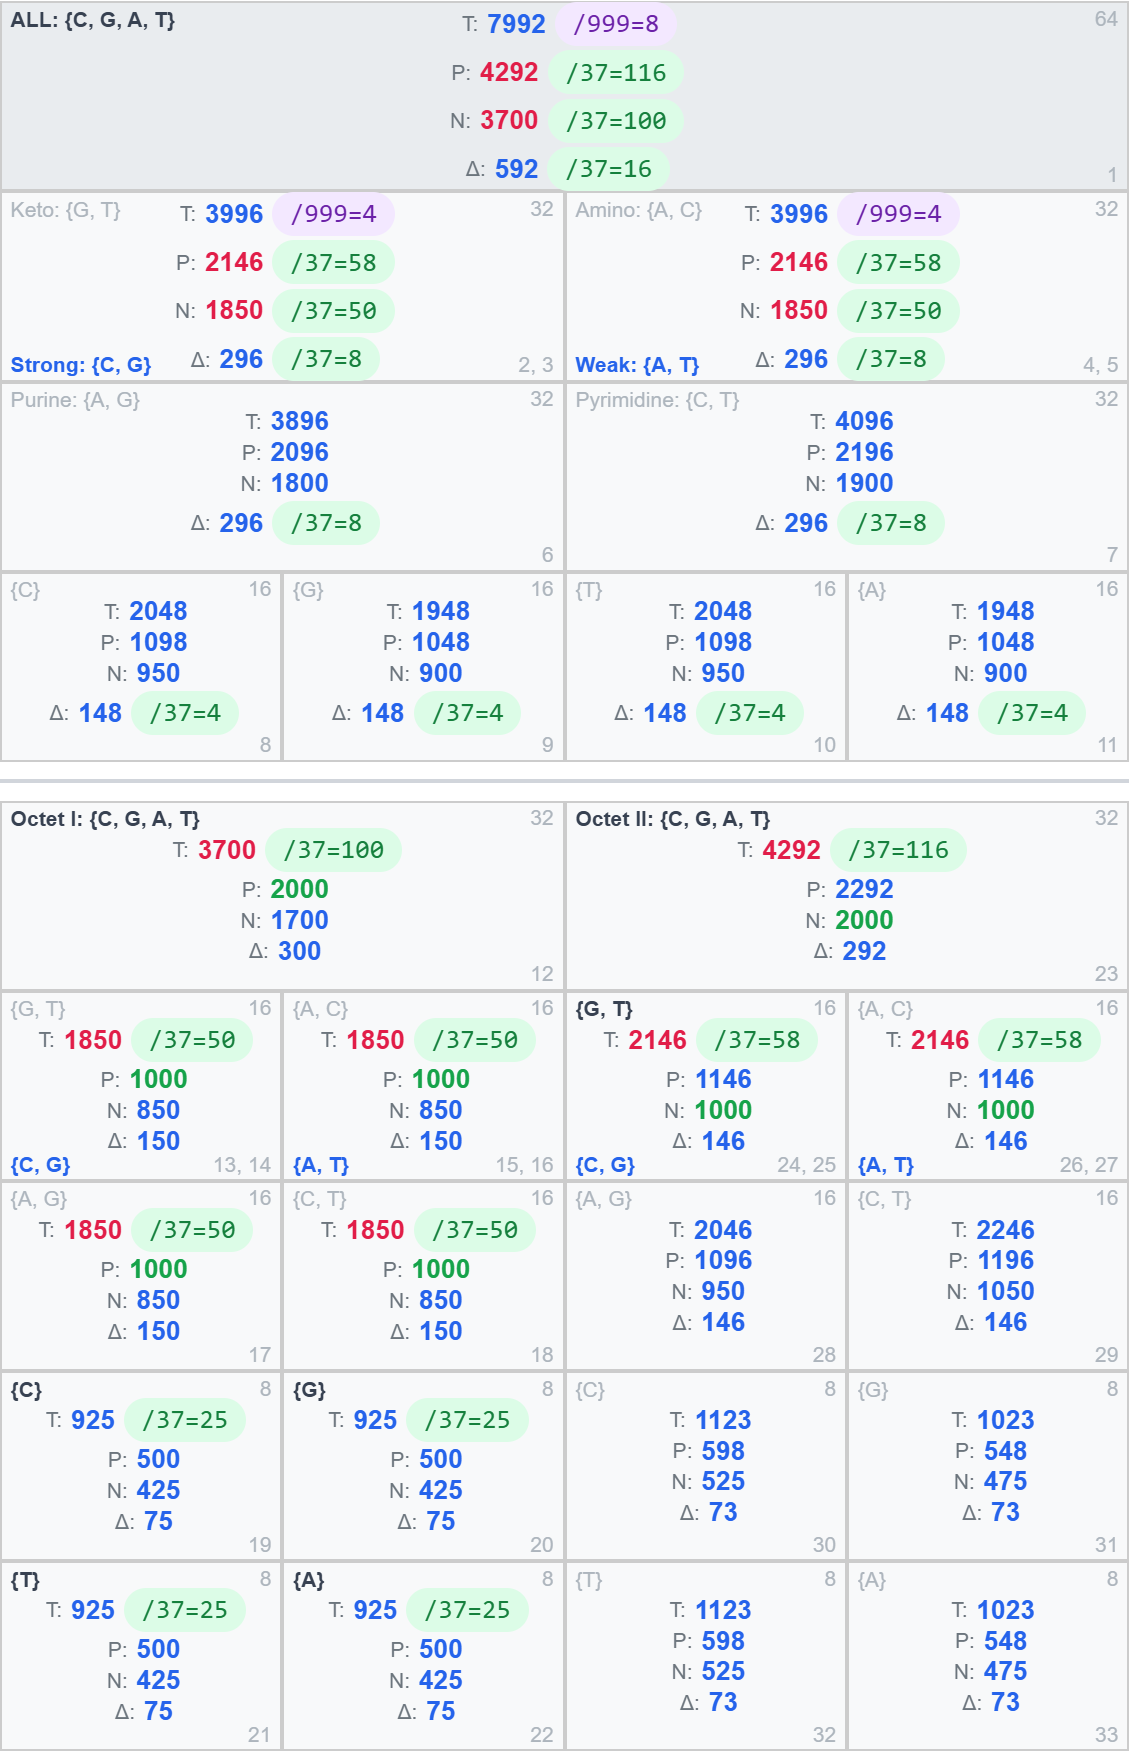
\includegraphics[width=0.78\textwidth]{groups_key1.png}
\caption{Nucleon sums of codon groups under Key~1:
each stop codon is assigned $(P,N)=(37,37)$,
and the initiator $\mathrm{ATG}$ is assigned $(P,N)=(1,0)$.
The group layout and divisibility color code are the same
as in Figure~\ref{fig:pool60}; the comparison with Key~0
is shown in Figure~\ref{fig:groups-key0}.
Generated with the accompanying visualizer
\texttt{visualization.html}.}
  \label{fig:groups-key1}
\end{figure}

\subsubsection{Alignment of the chemical-axis \texorpdfstring{$32$}{32}-codon groups}
\label{sec:results-key1-axisalignment}

Under Key~1, Keto, Amino, Strong, and Weak have identical
values of the four nucleon quantities:
\[
T=3996,\qquad P=2146,\qquad N=1850,\qquad \Delta=296.
\]
Keto/Amino balance ensures equality of the sums of all
four groups in $P$ and $N$, while the definitions
$T=P+N$ and $\Delta=P-N$ ensure equality in $T$ and $\Delta$. Thus the four aligned groups are a
consequence of the chosen assignment, rather than four
separate confirmations. Their sums are half those of the
complete table. All group values are given in
\texttt{key1\_nucleon-data.csv}.

Purine and Pyrimidine have the same $\Delta$ but differ
in $P$, $N$, and $T$. This difference is examined in
Section~\ref{sec:results-key1-purpyr}.

\subsubsection{Macroscopic identities and propagation to chemical-axis halves}
\label{sec:results-key1-macroidentities}

The relation between the complete table and the octets
has three equivalent forms:
\begin{align*}
N_1(\mathrm{All})
&=T(\mathrm{Octet~I})=3700=100\cdot37,\\
P_1(\mathrm{All})
&=T_1(\mathrm{Octet~II})=4292=116\cdot37,\\
N_1(\mathrm{Octet~II})
&=P(\mathrm{Octet~I})=2000=2\cdot1000.
\end{align*}
This is one relation, obtained in
Section~\ref{sec:results-key1-neutrons} after determining
the parameters. Subtracting $N(\mathrm{Octet~I})=1700$
from the first equality gives the third. Adding
$P_1(\mathrm{Octet~II})$ to the third gives the second,
since $T=P+N$. The transformations also hold in reverse.
The sums of Octet~I are independent of parametrization;
those of Octet~II include the service-codon assignments.

For each of the four aligned groups $G$---Keto, Amino,
Strong, and Weak---this relation is reproduced at the
level of its octet intersections:
\[
\begin{aligned}
N_1(G)&=T(G\cap\mathrm{Octet~I})=1850,\\
P_1(G)&=T_1(G\cap\mathrm{Octet~II})=2146,\\
N_1(G\cap\mathrm{Octet~II})
&=P(G\cap\mathrm{Octet~I})=1000.
\end{aligned}
\]
Each intersection contains $16$ codons. In Octet~I,
each such group includes two codons from every four-fold
degenerate family and therefore carries half the octet
sums. In Octet~II, equality of the halves along the two
axes follows from complete-table balance after subtracting
the equal contributions of Octet~I. The equalities above
are therefore half-scale forms of the same relation.
This alignment of Octet~II does not hold for Purine and
Pyrimidine. The complete list of equalities is given in
\texttt{key1\_equalities.csv}.

\paragraph{Rational profile.}
The complete table and the four aligned groups share
the same ratios of nucleon quantities:
\[
\frac{P}{T}=\frac{29}{54},\qquad
\frac{N}{T}=\frac{25}{54},\qquad
\frac{\Delta}{T}=\frac{2}{27},\qquad P:N=29:25.
\]
This is a normalized expression of the same sums. For
each of the four groups, $2146=29\cdot2\cdot37$ is both
the proton sum of the group and the nucleon sum of its
intersection with Octet~II; $1850=25\cdot2\cdot37$
links the neutron sum to the intersection with Octet~I.
The ratio profiles of all groups are given in
\texttt{key1\_ratios.csv}.

\subsubsection{Divisibility by~\texorpdfstring{$37$}{37} and by~\texorpdfstring{$999$}{999}}
\label{sec:results-key1-divisibility37and999}

\paragraph{Divisibility by $37$.}
In the main derivation of Key~1, divisibility of the
total sums in $P$ and $N$ is explicitly imposed. For
neutrons it already holds at the minimal assignment
satisfying balance alone; for protons it changes the
minimum (Section~\ref{sec:results-key1-uniqueness}).
The resulting sums are
\[
N_1(\mathrm{All})=100\cdot37,\qquad
P_1(\mathrm{All})=116\cdot37.
\]
Balance divides each sum into two equal integer parts.
Since $37$ is odd, both parts are also divisible by
$37$. Each of the four aligned groups has
\[
T=108\cdot37,\quad P=58\cdot37,\quad
N=50\cdot37,\quad \Delta=8\cdot37.
\]
Divisibility of $T$ and $\Delta$ follows by adding and
subtracting $P$ and $N$; in particular,
$\Delta_1(\mathrm{All})=4292-3700=592=16\cdot37$.

A more general property holds for the nucleon sum:
\[
T_1(G)\equiv T_0(G)\pmod{37}
\]
for any codon group $G$. In the transition from Key~0
to Key~1, the contribution of each stop codon to $T$
increases by $74=2\cdot37$, whereas that of
$\mathrm{ATG}$ changes by $1-149=-148=-4\cdot37$.
Divisibility of $T$ by $37$ is therefore preserved in
this transition regardless of the group's composition.
The divisibility records under Key~1 are given in
\texttt{key1\_divisibility-37.csv}.

\paragraph{Divisibility by $999$.}
The total nucleon sum has the form
\[
T_1(\mathrm{All})=7992=8\cdot999=6^3\cdot37.
\]
Unlike divisibility by $37$, divisibility by
$999=27\cdot37$ was not imposed as a separate condition.
It characterizes the minimal solution obtained.
Each of the four aligned halves has
$T=3996=4\cdot999$; this follows by halving the total
sum and is not another numerical coincidence.

\subsubsection{The \texorpdfstring{$\Delta$}{Delta}-invariant across all six \texorpdfstring{$32$}{32}-codon groups}
\label{sec:results-key1-deltainvariant}

Under Key~1, all six third-position $32$-codon groups
have the same proton-neutron difference:
\[
\begin{aligned}
\Delta_1(\mathrm{Keto})=\Delta_1(\mathrm{Amino})
&=\Delta_1(\mathrm{Strong})=\Delta_1(\mathrm{Weak})\\
&=\Delta_1(\mathrm{Purine})=\Delta(\mathrm{Pyrimidine})=296.
\end{aligned}
\]
For the first four groups, equality follows from balance
in $P$ and $N$. Equality of Purine and Pyrimidine in
$\Delta$ is not imposed separately in the main
derivation; in the alternative two-axis derivation it
serves as a condition in place of divisibility
(Section~\ref{sec:results-key1-uniqueness}). Its role
therefore differs between the two derivations.

The common difference is reproduced at lower levels
of partitioning. Every eight-codon group of Octet~I
selected by a single nucleotide in the third position
has $\Delta=75$ independently of parametrization
(Section~\ref{sec:results-octetI}). Under Key~1, every
corresponding group of Octet~II has $\Delta=73$:
\[
\Delta(G_X\cap\mathrm{Octet~I})=75,\qquad
\Delta_1(G_X\cap\mathrm{Octet~II})=73
\qquad (|X|=1).
\]
In the pyrimidine groups, $73$ is also independent of
parametrization (Section~\ref{sec:results-pyrimidine});
in the purine groups it is attained under the derived
assignment. Adding two eight-codon groups within each
octet gives
\[
\Delta(G_X\cap\mathrm{Octet~I})=150,\qquad
\Delta_1(G_X\cap\mathrm{Octet~II})=146
\qquad (|X|=2).
\]
Adding across the octets gives, for each one-nucleotide
group of the complete table,
\[
\Delta_1(G_X)=75+73=148=4\cdot37
\qquad (|X|=1).
\]
Under Key~0, the $\{\mathrm{G}\}$ group had
$\Delta_0(\{\mathrm{G}\})=158$, whereas the other
three already had $148$
(Section~\ref{sec:results-key0-delta}). Under Key~1,
all four values coincide. Both routes of addition
reach the $32$-codon level:
\[
296=2\cdot148=150+146.
\]
Thus the cascade describes one agreement at several
levels. It also persists for nonminimal assignments
in the two-axis family of
Section~\ref{sec:results-key1-uniqueness}: increasing
both parameters by the same amount leaves $\Delta$
unchanged for every service codon.

\subsubsection{Purine/Pyrimidine asymmetry}
\label{sec:results-key1-purpyr}

Under Key~1, the Purine/Pyrimidine axis retains the
following differences between the sums of its halves:
\begin{align*}
N(\mathrm{Pyrimidine})-N_1(\mathrm{Purine})&=100,\\
P(\mathrm{Pyrimidine})-P_1(\mathrm{Purine})&=100,\\
T(\mathrm{Pyrimidine})-T_1(\mathrm{Purine})&=200,\\
\Delta(\mathrm{Pyrimidine})-\Delta_1(\mathrm{Purine})&=0.
\end{align*}
The entire asymmetry lies in Octet~II: in Octet~I,
the purine and pyrimidine halves have equal sums
because its families are four-fold degenerate.

In the service-excluded pool, the Pyrimidine--Purine
differences are $212$ in $P$ and $211$ in $N$
(Section~\ref{sec:results-sensepool}). Key~1 adds
$112$ protons and $111$ neutrons to the purine half,
so
\[
212-112=211-111=100.
\]
Equality of the two shifts is equivalent to equality
of $\Delta$ between Purine and Pyrimidine. Their common
magnitude of $100$ is obtained from the initial sums
after assigning the parameters; it was not imposed
as a condition of the derivation.

\paragraph{Equalities at the one-nucleotide level.}
Equality of the sums of the $\{\mathrm{C}\}$ and
$\{\mathrm{T}\}$ groups is independent of
parametrization and follows from pyrimidine synonymy
(Section~\ref{sec:twin-identities}). Since Keto combines
$\{\mathrm{G}\}$ and $\{\mathrm{T}\}$, whereas Amino
combines $\{\mathrm{A}\}$ and $\{\mathrm{C}\}$,
balance in $P$ and $N$ gives
\[
P_1(\{\mathrm{G}\})=P_1(\{\mathrm{A}\}),\qquad
N_1(\{\mathrm{G}\})=N_1(\{\mathrm{A}\}).
\]
This restates balance and holds for any assignment
that satisfies it. Under Key~1, the two pairs of
groups have the values
\[
\begin{aligned}
\bigl(T(\{\mathrm{C}\}),P(\{\mathrm{C}\}),N(\{\mathrm{C}\})\bigr)
&=(2048,1098,950),\\
\bigl(T_1(\{\mathrm{G}\}),P_1(\{\mathrm{G}\}),N_1(\{\mathrm{G}\})\bigr)
&=(1948,1048,900),
\end{aligned}
\]
with the same values for $\{\mathrm{T}\}$ and
$\{\mathrm{A}\}$, respectively. The difference between
the pairs is $50$ in $P$ and $N$ and $100$ in $T$;
doubling reproduces the differences between the two
$32$-codon halves. Subtracting the equal Octet~I
contributions leaves $T=1023$, $P=548$, $N=475$
in each of the groups
$\{\mathrm{G}\}\cap\mathrm{Octet~II}$ and
$\{\mathrm{A}\}\cap\mathrm{Octet~II}$ under Key~1.

\paragraph{Inside Octet~II at the $16$-codon level.}
The purine and pyrimidine halves of Octet~II have
neutron sums of $950$ and $1050$ and proton sums of
$1096$ and $1196$, respectively. They deviate by
$\pm50$ from the mean values $N=1000$ and $P=1146$
of the halves of this octet along the Keto/Amino and
Strong/Weak axes. This is another expression of the
same asymmetry: the two halves lie symmetrically about
the mean but are not equal to each other.

\paragraph{The limit of alignment.}
The residual asymmetry does not imply that complete
balance across the three axes is impossible. In the
two-axis family of Section~\ref{sec:results-key1-uniqueness},
where the stop codons have parameters $(37+t,37+t)$
and the initiator has $(1+t,t)$, both
Pyrimidine--Purine shifts equal $100-4t$. At $t=25$,
the assignments $(62,62)$ to the stop codons and
$(26,25)$ to the initiator equalize all six halves
in $P$ and $N$. However, the total sums become
$P=4392$ and $N=3800$ and are not divisible by $37$;
the neutron equality with $T(\mathrm{Octet~I})=3700$
is also lost. Key~1 fixes the minimal reconciliation
of balance with divisibility, retaining this asymmetry.

\subsection{Synthesis}
\label{sec:results-synthesis}

The observed regularities connect two levels of organization
of the standard genetic code: the structure of codon groups
and the nucleon composition of the encoded amino acids.
The partitions are based on the chemical properties of bases,
pyrimidine synonymy, and Rumer's octets. In the adopted
representation of free neutral amino acids, proton and neutron
counts are uniquely determined by molecular composition,
while group sums account for the number of codons encoding
each amino acid. The choice of the third position, molecular
representation, and modulus~$37$ defines the analytical
framework; these choices alone do not entail the observed
numerical values.

The structural partitions exhibit arithmetic agreement
even before values are assigned to service codons.
In Octet~I, the proton and neutron sums are $2000$ and $1700$,
and their sum, $3700=100\cdot37$, connects a decimal scale
with modulus~$37$. The octet's structure ensures exact
scaling of these quantities across its groups but does not
determine their initial values. For the entire service-excluded
pool, the neutron sum is $3589=97\cdot37$, while the proton
sum is $4180=113\cdot37-1$
(Section~\ref{sec:results-independent}).

The local asymmetry agrees with this global pattern.
The difference between Keto and Amino reduces to the
tryptophan--isoleucine pair, whose differences are $37$
in neutrons and $36$ in protons. Among the $190$ pairs
of canonical amino acids, this combination of differences
occurs only for tryptophan--isoleucine and
tryptophan--leucine. The agreement is explained by
isoleucine and leucine being isomers with identical
nucleon counts
(Section~\ref{sec:results-key1-trpile}).
The even proton counts of all canonical amino acids
rule out a proton difference of $37$ but do not determine
how far the actual difference must deviate from it.
The value $36$ is the nearest permitted value below $37$,
and the proton and neutron imbalances differ by exactly
one unit
(Section~\ref{sec:results-proton-parity}).

One-unit deviations occur at different levels of the
structure and have different arithmetic origins.
In Octet~I, the values $75=2\cdot37+1$ arise by dividing
its difference $\Delta=300$ among four equal
eight-codon groups. In the pyrimidine groups of Octet~II,
the value is displaced in the opposite direction:
$73=2\cdot37-1$. When the octets are combined,
the deviations cancel: $75+73=148=4\cdot37$.
In the service-excluded pool, the $\{\mathrm{A}\}$ branch
of Octet~II also has $\Delta=73$, an equality that
does not follow from pyrimidine synonymy.
Only the $\{\mathrm{G}\}$ branch differs, with a value
of $72$; the excluded $\mathrm{ATG}$ position lies
in this branch
(Section~\ref{sec:results-key0-delta}).
A further agreement appears under Key~0:
methionine's nucleon count, $149=4\cdot37+1$,
compensates for the remainder of $-1$ in the pool's
nucleon sum. Thus, one-unit deviations have several
sources, and their recurrences propagate through
structural relations among groups.

The arrangement of service codons allows local balance
to be reconciled with global sums.
Keto contains one stop codon and $\mathrm{ATG}$,
whereas Amino contains two stop codons. With the same
assignment to all stop codons, the minimal non-negative
integer compensation for the neutron imbalance assigns
$37$ neutrons to each stop codon and zero to $\mathrm{ATG}$.
This gives
\[
N_1(\mathrm{All})=3589+3\cdot37
               =3700=T(\mathrm{Octet~I}).
\]
The coincidence with the Octet~I sum was not used
to select the compensation. Here, the magnitude of
the local imbalance, the number and arrangement of
stop codons, and the sum of structural Octet~I agree.

On the proton side, moving from the minimal balanced
assignment to the minimal balanced assignment with
divisibility by~$37$ requires four additional protons---
one for each service position.
Their equal distribution between Keto and Amino
preserves balance. Since all four positions belong
to Purine, the same increment eliminates the difference
in $\Delta$ between Purine and Pyrimidine while preserving
the original pyrimidine sums. The resulting assignment
is Key~1: $(P,N)=(37,37)$ for each stop codon and $(1,0)$
for $\mathrm{ATG}$
(Section~\ref{sec:results-key1-derivation}).
Its simplicity expresses the compatibility of the
initial numbers with the arrangement of service positions;
uniqueness is relative to the adopted conditions
and minimality criterion.

The resulting assignment brings these relations together
in the complete table. Several macroscopic equalities express a single relation
with Octet~I; equality of $\Delta$ is compatible with
Pyrimidine exceeding Purine by $100$ in both proton
and neutron sums. The nucleon sum $7992=8\cdot999$ adds
to the numerical profile, although divisibility by~$999$
was not imposed as a separate condition
(Section~\ref{sec:results-key1-consequences}).
The result concerns the agreement among molecular
counts, structural partitions, and formal assignments;
repeated manifestations of one relation do not constitute
separate pieces of evidence. The specificity of this
agreement is assessed next through comparison with
alternative codes, deterministic controls, and a null
model
(Section~\ref{sec:discussion}).

\section{Discussion}
\label{sec:discussion}

This section examines how far the regularities reported
above are specific to the standard code and its structure,
rather than artifacts of the analysis.
Section~\ref{sec:discussion-trpile-robustness} compares the
standard code against the alternative NCBI codes on the
sense-pool arithmetic, testing both the global alignment with
the $37$-lattice and the robustness of the
$\mathrm{Trp}$--$\mathrm{Ile}$ localization;
Section~\ref{sec:discussion-controls} asks whether the
third codon position and the modulus~$37$ are
distinguished from other positions and divisors; and
Section~\ref{sec:discussion-montecarlo} assesses the
concentration on the $37$-lattice against a random-code
null. Section~\ref{sec:discussion-prior-work} situates the
results relative to prior work, and
Section~\ref{sec:discussion-limitations} states the
limitations and outlook.

\subsection{Specificity across alternative genetic codes}
\label{sec:discussion-trpile-robustness}
\label{sec:results-key1-ncbi}

The standard genetic code is one of $27$ translation tables in the
NCBI registry. The parametrization-independent sense-pool arithmetic
of Section~\ref{sec:results-independent} admits direct comparative
tests across these tables: for each alternative code one can ask
whether the same arithmetic holds. Two such tests are reported here.
The first concerns the global alignment of the sense pool with the
lattice of step~$37$---the neutron deficit and the proton residue of
Section~\ref{sec:results-sensepool}. The second concerns the
localization of the Keto/Amino asymmetry in the single pair
$\mathrm{Trp}$--$\mathrm{Ile}$
(Section~\ref{sec:results-key1-trpile}). Both quantities are
properties of the sense pool and require no assignment to the service
codons; the closure of the first pair under Key~1 is a separate
matter, treated in Section~\ref{sec:results-key1-derivation}. The two
tests probe different aspects of the arithmetic and, as shown below,
identify different sets of matching alternative codes.

Because both tests depend on which codons are counted as stops, both
are computed under two model choices for the sense pool:
\begin{itemize}
  \item
    Sense pool, Model~1 (primary): all codons listed as stops in the
    NCBI registry are excluded, even when they are read as amino
    acids in context-dependent codes. The primary start codon
    $\mathrm{ATG}$ is excluded as the universal initiator. Initiation
    is a property of the first codon position rather than of the
    triplet itself, so exactly one initiator codon is removed;
    alternative start codons such as $\mathrm{GTG}$ and
    $\mathrm{TTG}$ carry their elongation meaning at every internal
    position and are counted as sense codons.
  \item
    Sense pool, Model~2 (alternative): in the three codes with
    context-dependent stops (Tables~$27$, $28$, $31$), codons that
    function as amino acids in mid-sequence and as stops at gene
    termini are treated as sense codons. For all other tables,
    Model~2 coincides with Model~1.
\end{itemize}
The model conventions are documented in the datasets accompanying
\texttt{deficit\_models\_analysis.csv} and
\texttt{keto\_amino\_balance\_models.csv}.

\paragraph{Global alignment of the sense pool with the lattice.}
The first test records two quantities of the sense pool: the neutron
deficit relative to a reference total,
$\Delta_N = T_{\mathrm{ref}} - N(\mathcal{C}_{\mathrm{SE}})$, and the
proton residue $P(\mathcal{C}_{\mathrm{SE}}) \bmod 37$. For the standard
code these are
$\Delta_N = T(\mathrm{Octet~I}) - N(\mathcal{C}_{\mathrm{SE}}) = 3700 - 3589
= 111 = 3 \cdot 37$ and $P(\mathcal{C}_{\mathrm{SE}}) \equiv -1 \pmod{37}$
(Section~\ref{sec:results-sensepool}); under Key~1 the first deficit
is closed by the three stop codons to align $N(\mathrm{All})$ with
the invariant $T(\mathrm{Octet~I})$, and the proton residue by the
start-codon parameter $p_{\text{start}} = 1$. For the neutron
deficit, three model choices of $T_{\mathrm{ref}}$ are considered:
the constant $T(\mathrm{Octet~I}) = 3700$ of the standard code, the
total nucleon content of the eight structural Octet~I families under
the amino-acid assignments of the specific table, and the total
nucleon content of all $4$-fold degenerate codon families in the
specific table. For the proton residue the relevant quantity is
intrinsic to the sense pool and requires no reference total. The full
set of computed values across all tables and model combinations is
tabulated in \texttt{deficit\_models\_analysis.csv}.

The two records give parallel outcomes: in each, the arithmetic
property holds in exactly the same three tables. Table~$1$ (the
standard code) and Table~$11$ (the Bacterial, Archaeal and Plant
Plastid Code) have $\Delta_N = 111 = 3 \cdot 37$ under all three
reference models and $P(\mathcal{C}_{\mathrm{SE}}) \equiv -1 \pmod{37}$
under both sense-pool models; their amino acid assignments are
identical and they share the same set of stop codons, so
arithmetically they are the same code applied in different domains.
Table~$28$ (the Condylostoma Nuclear Code) gives the same values as
the standard code under Model~$1$ and different values under
Model~$2$: its three context-dependent stop codons, once excluded
alongside $\mathrm{ATG}$, leave a sense codon set identical to the
one used for the standard code, whereas under Model~$2$ they are
returned to the pool and neither the deficit nor the residue matches.
In the remaining $24$ tables neither property holds under any model
combination. That the two records identify the same tables reflects a
single underlying sense pool rather than independent agreement:
Tables~$1$, $11$, and (under Model~$1$) $28$ all share the standard
code's sense-codon assignments.

Across the $27$ tables, six reasonable definitions of the neutron
deficit and two of the proton residue, only the standard code and its
exact codon-to-amino-acid equivalent (Table~$11$) satisfy both
conditions under every model. Tables that reassign codons within the
structural Octet~I families, shift the set of $4$-fold-degenerate
families, or use a different number of stop codons destroy the match
between the sense pool and the lattice of step~$37$. The global
alignment is therefore not a generic feature of genetic codes.

\paragraph{Preservation of the Trp--Ile localization.}
The second test asks whether the localization of the Keto/Amino
asymmetry in the pair $\mathrm{Trp}$--$\mathrm{Ile}$ survives in
alternative codes. The relevant signature is the pair of sense-pool
differences $N_{\mathrm{SE}}(\mathrm{Keto}) - N_{\mathrm{SE}}(\mathrm{Amino}) = 37$
and $P_{\mathrm{SE}}(\mathrm{Keto}) - P_{\mathrm{SE}}(\mathrm{Amino}) = 36$, the
$(37, 36)$ signature; the values across all tables are computed in
\texttt{keto\_amino\_balance\_models.csv}. The signature is
reproduced exactly in seven tables. Five---Table~$1$ (Standard),
Table~$6$ (Ciliate, Dasycladacean and Hexamita Nuclear), Table~$11$
(Bacterial, Archaeal and Plant Plastid), Table~$29$ (Mesodinium
Nuclear), and Table~$30$ (Peritrich Nuclear)---reproduce it under
both sense-pool models; the remaining two, Table~$27$ (Karyorelict
Nuclear) and Table~$28$ (Condylostoma Nuclear), reproduce it only
under the primary interpretation of context-dependent stop codons.

The mechanism is structural and operates differently in different
tables. Table~$11$ has an amino acid assignment identical to the
standard code and shares its set of stop codons, so the signature
holds trivially. In Tables~$6$, $29$, and~$30$ the codons
$\mathrm{TAG}$ and $\mathrm{TAA}$ are reassigned to the same amino
acid ($\mathrm{Gln}$, $\mathrm{Tyr}$, or $\mathrm{Glu}$
respectively); since $\mathrm{TAG}$ sits in the Keto branch of family
$\mathrm{TA}$ and $\mathrm{TAA}$ in the Amino branch, this symmetric
reassignment contributes identically to both branches of the sense
pool and the Keto/Amino differences are preserved. No codons other
than $\mathrm{TAA}$ and $\mathrm{TAG}$ are reassigned in these tables;
in particular, neither $\mathrm{TGG}$ ($\mathrm{Trp}$) nor any codon
of $\mathrm{Ile}$ is changed, and the $\mathrm{Trp}$/$\mathrm{Ile}$
localization of Section~\ref{sec:results-key1-trpile} continues to
hold. Tables~$27$ and~$28$ involve context-dependent stop codons and
behave differently under the two models: Table~$28$ declares all
three of $\mathrm{TAA}$, $\mathrm{TAG}$, $\mathrm{TGA}$ as
context-dependent stops, so under Model~$1$ its sense pool is
identical to that of the standard code and the signature is
reproduced, while under Model~$2$ the three codons re-enter the pool
and it is lost; Table~$27$ permanently reassigns $\mathrm{TAA}$ and
$\mathrm{TAG}$ to $\mathrm{Gln}$ (the same symmetric mechanism) and
treats only $\mathrm{TGA}$ as a context-dependent stop, so Model~$1$
preserves the signature while Model~$2$, including $\mathrm{TGA}$ as
$\mathrm{Trp}$ in the Keto branch, breaks it. Tables that reassign
$\mathrm{ATA}$ (typically to $\mathrm{Met}$ in mitochondrial codes)
or $\mathrm{TGA}$ (typically from stop to $\mathrm{Trp}$) change the
amino acid content of the carrier codons and no longer reproduce the
signature.

The asymmetry between nuclear and mitochondrial codes is informative.
All seven tables matching the $(37, 36)$ signature are nuclear or
bacterial; none of the thirteen mitochondrial translation tables in
the NCBI registry reproduces it, the failure tracing in each case to
the reassignment of $\mathrm{ATA}$ or $\mathrm{TGA}$, both altering
codons on which the localization depends.

\paragraph{Relation between the two tests.}
A finer decomposition connects the seven matching tables to the first
test. In the standard code the four sense-pool half-quantities have
the residues
$(N_{\mathrm{Keto}}, N_{\mathrm{Amino}}, P_{\mathrm{Keto}},
P_{\mathrm{Amino}}) \equiv (0, 0, -1, 0) \pmod{37}$, an arithmetic
profile combining divisibility of each half-pool by~$37$ with a
one-unit proton residue: parity bars the proton half-pools from the
odd multiples of~$37$, and the specific nucleon counts place the
residue at exactly one. Tables~$1$, $11$, and
$28$ (under Model~$1$) reproduce all four residues exactly---for
Table~$11$ by identity with the standard code, for Table~$28$ under
Model~$1$ because its sense pool coincides with the standard once the
context-dependent stops are excluded---and these are exactly the
three tables that match in the global-alignment test above. The four
additional tables matching the $(37, 36)$ signature ($6$, $27$, $29$,
$30$) show a different profile: $N_{\mathrm{Keto}}$ and
$N_{\mathrm{Amino}}$ share the same non-zero residue mod~$37$, and
$P_{\mathrm{Keto}}$ and $P_{\mathrm{Amino}}$ differ by one unit, but
the absolute level has detached from the lattice. This is the
signature of symmetric reassignment of $\mathrm{TAA}$ and
$\mathrm{TAG}$ to a common amino acid: each half-pool acquires the
same non-zero contribution, so the Keto/Amino differences are
preserved while the divisibility of each half by~$37$ is lost. Among
the $27$ tables, $13$ preserve the divisibility of at least one
half-pool by~$37$, three of them mitochondrial (Tables~$4$, $16$,
and~$23$).

The global-alignment test measures the absolute
alignment of the whole sense pool with the $37$-lattice and matches
only tables arithmetically equivalent to the standard code in their
sense pool (Tables~$1$, $11$, and~$28$ under Model~$1$). The
localization test measures the preservation of a relational pattern
between the Keto and Amino branches and additionally matches tables
in which the only divergence from the standard code is a symmetric
reassignment of $\mathrm{TAA}$ and $\mathrm{TAG}$ (Tables~$6$, $27$,
$29$, $30$). Together they show that the parametrization-independent
sense-pool arithmetic of the standard code, in both its absolute and
its relational form, is specific to the standard code among the known natural codes,
holding elsewhere only in tables that are arithmetically equivalent
to it or differ from it by a symmetric reassignment of
$\mathrm{TAA}$ and $\mathrm{TAG}$.

\subsection{Specificity of the third codon position, the modulus~\texorpdfstring{$37$}{37}, and the molecular representation}
\label{sec:discussion-controls}

Two features are built into the framework of this work rather
than derived from the data: the three chemical axes are read
off the third codon position
(Section~\ref{sec:partitioning}), and divisibility by $37$ is
the primary criterion (Section~\ref{sec:criteria}). Two
deterministic controls test whether the observed structure is
specific to these two choices or would arise generically.

\paragraph{Codon position.}
Applying the same three chemical axes to the first and second
codon position, instead of the third, removes the structure
almost entirely. At the third position the Amino and Weak
groups have all four nucleon quantities divisible by $37$, the
Keto and Strong groups have their neutron pool divisible, and
the Pyrimidine group has $\Delta$ divisible. At the first
position the only divisibility is the neutron pool of the
Keto/Amino axis, present in both its complementary halves, and
this is not an independent fact: Keto and Amino are
complementary, so their sense-pool neutron counts sum
to $N(\mathcal{C}_{\mathrm{SE}}) = 3589 = 97 \cdot 37$
(Section~\ref{sec:results-key1-neutrons}), and divisibility of
one half forces divisibility of the other. At the second
position no nucleon quantity of any axis is divisible by $37$.
The control thus shows that divisibility by $37$ along the
chemical axes is confined to the third codon position: the same
axes applied to the first and second positions do not meet the
$37$-lattice, the single first-position exception being the
dependent one noted above. This excludes the alternative in
which any equal-size split of the sense pool into chemical halves
would align with the $37$-lattice irrespective of position. The full values for all three positions are
tabulated in \texttt{position\_axis\_analysis.csv}.

\paragraph{Choice of modulus.}
For every prime up to $97$ we count how many of the four
nucleon quantities of the codon groups it divides, over three
value sets: the parametrization-independent groups (those with
no service codon, on which $37$ cannot be imposed), the groups
under Key~0 (which does not impose $37$), and the groups under
Key~1 (whose derivation does). The scan ranges over primes
rather than all integers because divisibility by a composite is
the conjunction of divisibilities by its prime-power factors and
introduces no new modulus, and because raising a prime to a
higher power lowers the chance rate $1/m$ and thereby inflates
the excess over the same quantities without adding information;
the prime is the appropriate unit. The informative statistic is
accordingly the excess over the chance rate $1/p$, computed over
distinct values so that quantities forced to coincide by the
structure of the code are not counted more than once.

Three primes divide their share at essentially the chance rate
($3$, $7$ and $13$). Two exceed it modestly, by less than a factor of three across the three value sets: $2$, because every canonical amino acid has an even proton count (Section~\ref{sec:results-proton-parity}), and $5$,
reflecting the round-number regularity already reported in
Section~\ref{sec:results-synthesis}, which the scan thus
corroborates. Against this background $37$ divides five of the
twenty-eight distinct parametrization-independent quantities,
thirteen of the seventy distinct Key~0 quantities, and ten of
the forty-seven under Key~1 --- in each case several times the
naive rate $1/37$. This excess ratio is descriptive, not a
$p$-value: the scan is deterministic and has no null model, and
the nested group hierarchy makes the quantities non-independent,
so the ratio alone cannot be read as a significance. An additional
descriptive distinction not captured by that ratio is that the
multiples of $37$ contain several distinct odd cores, whereas the
comparable factors $73$ and $61$ each reduce to a single core. Because the
effect is already present in the value sets where $37$ is not
imposed, it is in any case not an artifact of the Key~1
derivation.

Three features set $37$ apart from the two small primes, all
independent of the number base. It is a larger prime, so each
divisible quantity is rarer under the null. It has no structural
counterpart to proton parity. And, unlike $5$ --- whose
multiples in these value sets are almost all multiples of $25$,
so that the larger excess one would attribute to $25$, $50$ or
$100$ only re-scores the same quantities against a smaller chance
rate --- the modulus $37$ occurs at a single power: no quantity
is divisible by $37^2$, so its excess does not grow when the
modulus is enlarged. Reducing each quantity to its odd part ---
dividing out the powers of two that the nested group hierarchy
(Octet~I and its sixteen- and eight-codon sub-groups) introduces
mechanically, since a group of size $2k$ has twice the nucleon
counts of its size-$k$ refinement --- sharpens this. Among the
Key~0 quantities, $37$ divides ten distinct odd cores; the
multiples of $73 = 2 \cdot 37 - 1$ (the value of $\Delta$ for
the Octet~II eight-codon groups) collapse to that single core,
and the multiples of $61$ to the single core $549 = 9 \cdot 61$,
to which the pyrimidine proton pool
$P(\mathrm{Pyrimidine}) = 2196 = 2^2 \cdot 3^2 \cdot 61 = 4 \cdot 549$
and the proton count of each pyrimidine letter
$1098 = 2 \cdot 549$ both reduce. The factor $73$ is thus an echo of the modulus
itself; the factor $61$ is an isolated factorization unrelated
to $37$ (its quantities deviate from the nearest multiples of
$37$ by $+13$ and $-12$, not by $\pm1$ or $\pm2$); and the
factor $5$ reduces entirely to $10$ and $25$, every quantity
here divisible by $5$ being divisible by $10$ or by $25$. The
odd-core counts are tabulated in the corresponding column of
\texttt{prime\_divisibility\_scan.csv}.

\paragraph{Representation dependence and the invariant relational core.}
The nucleon counts throughout are those of the free (neutral) amino acids --- the canonical molecular identity of the species each codon encodes --- under the most-abundant-isotope convention ($^{1}\mathrm{H}$, $^{12}\mathrm{C}$, $^{14}\mathrm{N}$, $^{16}\mathrm{O}$, $^{32}\mathrm{S}$). Any alternative representation of the encoded amino acid differs from this one by a fixed nucleon offset per residue: the peptide residue removes one water ($10$ protons, $8$ neutrons), the zwitterion removes nothing. Under such a uniform offset $(s_P, s_N)$, a linear combination of the counts is invariant if and only if its signed codon coefficients sum to zero; the control \texttt{representation\_sensitivity.csv} records every anchor under all three representations. This splits the regularities in two. The relational regularities --- the neutron and proton differences of the localizing pair $\mathrm{Trp}$--$\mathrm{Ile}$ ($|\delta N| = 37$, $|\delta P| = 36$) and the Keto/Amino and Strong/Weak axis differences ($37$, $36$) --- are differences between codon sets of equal cardinality and are therefore invariant under every such re-representation. The absolute regularities --- the sense-pool sums $N(\mathcal{C}_{\mathrm{SE}}) = 97 \cdot 37$ and $P(\mathcal{C}_{\mathrm{SE}}) \equiv -1 \pmod{37}$, the deficit $111 = 3 \cdot 37$, and the divisibility of the individual axis half-pools --- are not: a uniform offset preserves the neutron alignment only when $60\,s_N \equiv 0 \pmod{37}$, i.e., $s_N \equiv 0$ (since $\gcd(60, 37) = 1$), which among the representations considered excludes the peptide residue, while the neutral and zwitterionic forms of the free amino acid have the same elemental composition and therefore the same nucleon counts; under the peptide residue the sums become $N = 3109 \equiv 1$ and $P = 3580 \equiv 28 \pmod{37}$. The absolute alignment is therefore a property of the standard code's assignment in the canonical free-amino-acid representation, fixed a priori by molecular convention rather than by tuning, while the relational structure --- the load-bearing part of the analysis --- is representation-independent.

\paragraph{The functional-group asymmetry across positions.}
One observation on the Keto/Amino axis reaches beyond the third
position. The asymmetry $N(\mathrm{Keto}) - N(\mathrm{Amino})$
that localizes to the Trp--Ile pair at the third position
(Section~\ref{sec:discussion-trpile-robustness}) equals $37$
there; the same Keto/Amino axis --- the $\{G,T\}$ versus
$\{A,C\}$ split --- yields a quantity divisible by $37$ at the
first position as well ($N$-asymmetry $-333 = -9 \cdot 37$) and
at the second ($T$-asymmetry $185 = 5 \cdot 37$). The divisible
quantity is $N$, $T$, $N$ by position, fixed after inspection
rather than in advance, so this is a single observation along
one axis rather than a control of the kind above. The three are
arithmetically independent: each is a sum over a different
partition of the same sixty codons, and the divisibility at one
position neither follows from nor implies it at another; what
they share is only the choice of axis. Across the $27$ NCBI
translation tables, the result depends on the sense-pool model.
Under Model~1, the full three-position signature occurs for
Tables~1, 11, and 28, whereas under Model~2 it occurs only for
Tables~1 and 11. Table~28 is not an independent replication
under Model~1: after its three context-dependent stop codons are
excluded, its analyzed pool is identical to that of the standard
code. Thus, in neither model is the full signature reproduced by
a table with a non-equivalent analyzed pool. Apart from these full
matches, no table reaches more than one position. In particular,
Tables~6, 29, and 30 reach only the third position under both
models, whereas Table~27 reaches only the third position and only
under Model~1. Three caveats further qualify it. Unlike the
third-position case, the first- and
second-position asymmetries do not localize to a single
amino-acid pair --- each receives contributions from nineteen
of the twenty amino acids, because the cancellation that
isolates Trp and Ile relies on third-position synonymy, which
the other positions lack. Their non-divisible components carry
no analogue of the parity-induced residue $-1$ that
accompanies the third-position value. And, as in
Section~\ref{sec:discussion-trpile-robustness}, the $27$ tables
are not statistically independent, so this is evidence of
specificity among natural codes rather than of improbability
under a null model. The per-table values are tabulated in
\texttt{position\_asymmetry\_ncbi.csv}.

All four controls are deterministic, use exact integer
arithmetic, and are regenerated by \texttt{controls.py}
(Section~\ref{sec:datasets}).

\subsection{Significance under a random-code null}
\label{sec:discussion-montecarlo}

The controls of Section~\ref{sec:discussion-controls} show that
divisibilities concentrate in third-position groupings and that
modulus $37$ stands out among the tested prime moduli; the
comparison of Section~\ref{sec:discussion-trpile-robustness} shows
that, among the $27$ NCBI translation tables, the tested combination
occurs only in the standard code and its exact codon-to-amino-acid
equivalent. Specificity among realized codes,
however, is not improbability under an explicit null. We therefore
test the standard code against a random-code null of the kind
used in studies of genetic-code optimality
\citep{freeland1998}: the architecture of
the code is held fixed (the $64$ codons, the synonymous blocks
with their sizes, the three stop codons, the Rumer partition,
and the third-position axes), and the only thing randomized is
which amino acid, carrying its fixed proton and neutron counts,
occupies each of the twenty blocks. A trial is a uniformly random
permutation of the twenty real paired proton and neutron profiles
over the twenty synonymous blocks. The modulus $37$ is taken a
priori from the prior literature; the statistical summaries were
formally defined before the final Monte Carlo run. Because the
analysis was not preregistered before inspection of the observed
structure, the results are interpreted as exploratory.

S1--S3 and S4sense are evaluated over the sixty-codon sense pool
without assigning any values to service codons. S4sense averages
the distances to the nearest multiple of $37$ for the four
quantities $T$, $P$, $N$, and $\Delta$ over all $33$ groups, for
$132$ distances in total. Under S4a the stop codons contribute zero,
while the contribution at $\mathrm{ATG}$ in each random code is the
profile of the amino acid assigned by the permutation to the
$\mathrm{ATG}$ block. Under S4b each random code receives its own
minimal non-negative Key~1, re-derived by the same Keto/Amino balance
and global divisibility conditions used for the standard code.

For every statistic the Monte Carlo tail probability is calculated
as $p_{\mathrm{MC}}=(b+1)/(M+1)$, where $b$ is the number of random
codes at least as extreme as the standard code and $M=10^{6}$. A
$95\%$ Monte Carlo uncertainty interval is reported with each
estimate. The computation is reported in
\texttt{mc\_significance.py} and summarized in
\texttt{mc\_significance.csv}. An independent implementation, using
a different construction of the codon groups, a direct search for
Key~1, and a different random seed, reproduces the observed
statistics and tail probabilities within the expected Monte Carlo
error (\texttt{verify\_mc.py}).

Six statistical summaries are considered. S1 tests the joint
divisibility of two anchors:
$N(\mathcal{C}_{\mathrm{SE}}) = 3589 = 97 \cdot 37$ and
$T(\mathrm{Octet~I}) = 3700 = 100 \cdot 37$. Both events occur in
a fraction $0.000800$ of random codes (Monte Carlo $95\%$ interval
$0.000746$--$0.000856$). This is the directly estimated joint
probability; no assumption that the two events are independent is
used in its calculation.

S2 counts divisibility by $37$ among the four quantities $T$, $P$,
$N$, and $\Delta$ for nine sense-pool groups: the full pool, the
six chemical-axis half-pools, and the two octets. The standard code
has $13$ divisible quantities among $36$ nominal entries, against a
null mean of $1.0299$. A value of $13$ or greater occurred in $39$
of $10^{6}$ trials, giving
$p_{\mathrm{MC}} = 4.0 \times 10^{-5}$ with a $95\%$ interval of
$2.9 \times 10^{-5}$--$5.3 \times 10^{-5}$. The components of the
count are dependent: $T=P+N$, $\Delta=P-N$, and the Keto/Strong and
Amino/Weak groups form exact twin pairs. These dependencies are
reproduced in every permutation and are therefore already included
in the null distribution of the composite statistic.

S3 applies the same count to the $17$ groups that contain no
service codon at all, giving $68$ nominal entries. The standard code
has $14$ divisible quantities against a null mean of $2.1311$,
$p_{\mathrm{MC}} = 0.025135$, and a $95\%$ interval of
$0.024829$--$0.025443$. Eleven of the fourteen divisibilities are
structural copies of $T(\mathrm{Octet~I}) = 100 \cdot 37$, while
the remaining three form the pyrimidine $\Delta$-cascade
($\Delta(\mathrm{Pyrimidine}) = 8 \cdot 37$ and
$\Delta(\{\mathrm{C}\}) = \Delta(\{\mathrm{T}\}) = 4 \cdot 37$).
S3 therefore records the propagation of two structural cascades
and is treated as a secondary summary.

S4sense measures not only exact divisibility but the overall
proximity of the sense pool to the lattice of step $37$. For each
of the $33$ groups, the distances of $T$, $P$, $N$, and $\Delta$ to
the nearest multiple of $37$ are averaged, with zero included as a
distance of zero; $132$ quantities are included in total. The
standard code has mean distance $4.8182$ against a null mean of
$9.1495$. An equal or smaller distance occurs in a fraction
$0.000274$ of random codes, with a $95\%$ interval of
$0.000242$--$0.000307$. This statistic assigns no values to service
codons. Because the summary was defined after inspection of the
observed structure, it is treated as an exploratory continuous
sensitivity analysis.

S4a applies the same distance under Key~0. In the standard code
$\mathrm{ATG}$ encodes methionine; in each random code its
contribution is the amino acid actually assigned by the permutation
to the $\mathrm{ATG}$ block, while the stop codons contribute zero.
The standard code has mean distance $5.5606$ against a null mean of
$9.0157$, $p_{\mathrm{MC}} = 0.002807$, and a $95\%$ interval of
$0.002704$--$0.002912$. The concentration is therefore already
present under the naive Key~0, although Key~0 remains a formal
assignment of service-codon values.

S4b tests the Key~1 derivation symmetrically: the standard code and
every random code are evaluated under their own minimal
non-negative key, derived from the Keto/Amino balance and global
divisibility by $37$. The fixation of this axis and the compatibility
of the conditions are established in
Section~\ref{sec:results-key1-uniqueness}. The standard code has
mean distance $4.6364$ against a null mean of $7.7397$,
$p_{\mathrm{MC}} = 0.021106$, and a $95\%$ interval of
$0.020825$--$0.021389$. Thus the standard code's Key~1 is
moderately atypical among keys re-derived for random codes.

The two most sensitive sense-pool summaries --- the discrete S2
and the continuous S4sense --- describe the same overall
concentration from different directions. Their $p$-values are
dependent and must not be multiplied or interpreted as two
independent lines of evidence. S1 records two individual anchors
of the structure, whereas the weaker S3 shows that restriction to
groups with no service positions leaves mainly the Octet~I and
pyrimidine-$\Delta$ cascades.

S4a and S4b address separate questions about the two formal
assignments to service codons. S4a shows that the concentration is
retained under the naive Key~0. S4b evaluates the entire Key~1
derivation rather than the fixed values of the standard key and
gives a more moderate tail probability. The assignment-free
sense-pool results therefore form the central statistical part of
the analysis, while S4a and S4b are secondary tests of its extension
to the complete table.

All reported $p_{\mathrm{MC}}$ values are nominal tail probabilities
for the individual statistics; no multiplicity correction across the
six statistics was applied.

The null model fixes the standard code's degeneracy architecture
and the real paired proton and neutron counts of the amino acids and
randomizes only their assignment to blocks. A different generative
model would give different probabilities. The modulus $37$, the
Rumer partition, and the chemical axes have substantive a priori
origins, but the choice of global statistical summaries was not
preregistered before inspection of the structure. The results
therefore characterize the exploratory atypicality of the standard
code under one explicit combinatorial model rather than confirming
a preregistered hypothesis. Improbability under this null concerns
combinatorial codes, a different question from specificity among the
$27$ natural codes in
Section~\ref{sec:discussion-trpile-robustness}; it speaks to no
biological mechanism.

\subsection{Relation to prior work}
\label{sec:discussion-prior-work}

Three prior contributions are particularly relevant
to the arithmetic structure analyzed in this work.
Yu.~B.~Rumer~\cite{rumer1966,rumer1968} introduced the
partition of the $64$ codons of the standard code into
two equal classes: Octet~I
consisting of the eight fully degenerate families, and
Octet~II consisting of the eight
heterogeneous families. The two classes are related by
the involution
$R = (\mathrm{T} \leftrightarrow \mathrm{G},
\mathrm{C} \leftrightarrow \mathrm{A})$, under which
each family of one class is mapped to a family of the
other. Shcherbak and Makukov~\cite{makukov2013}
observed that the number~$37$ plays a recurrent role
in the genetic code, appearing as a divisor of amino acid nucleon sums
across various groupings of codons. Panov and Filatov~\cite{panov2024}
revisited and extended this analysis. They introduced
the per-codon counting rule, in which each of the $64$
codons contributes independently the nucleon count of
the amino acid it encodes. They also proposed that stop codons be assigned a
total nucleon count of~$74$ each rather than zero.

The present work differs from these in several
methodological choices. Shcherbak and Makukov, and
Panov and Filatov following them, decompose each amino
acid into a constant part with nucleon count~$74$ and
a variable side chain, and many of their nucleon sums
are formed over side chains alone. This decomposition
forces a special treatment of proline, whose
cyclic side chain reduces the nucleon count of its
constant part to~$73$ rather than~$74$: to bring it in line with
the other nineteen amino acids, Shcherbak and Makukov
introduce a virtual transfer of one nucleon from its
side chain to its constant part, an operation they
call the \emph{activation key}. The present work uses
full amino acid nucleon counts without separation into
constant and side-chain components, and the question
of how to treat proline does not arise. Shcherbak and
Makukov also adopt a counting rule in which each amino
acid contributes once per codon family rather than
once per codon; Panov and Filatov replace this with
the per-codon rule, which the present work also uses.
Finally, all nucleon sums in the prior works are
formed over the total nucleon count~$T$ (or over its
restriction to side chains); the separation of $T$
into protons~$P$ and neutrons~$N$, and the analysis of
the difference $\Delta = P - N$, are introduced in the
present work and underlie a class of arguments
unavailable when only $T$ is considered.

The two prior works also differ from ours in the
systematics by which codons are grouped. They apply
several different grouping schemes in parallel
(Gamow's sorting and others), each tailored to a
particular set of patterns. The present work formulates
a single grouping system based on the Rumer octets and
the third-position chemical axes, and analyzes the
arithmetic structure within it consistently. The
parametrization of service codons also differs:
Shcherbak and Makukov treat stop codons as contributing
zero and identify $\mathrm{ATG}$ with $\mathrm{Met}$
throughout, Panov and Filatov propose in addition the
assignment of total nucleon count~$74$ to stop codons
as an alternative, while the present work considers
the parametrization of service codons as part of the
derivation of Key~1
(Section~\ref{sec:results-key1-derivation}). Finally,
Shcherbak and Makukov work extensively with the
euplotid code variant (in which $\mathrm{TGA}$ is
reassigned to $\mathrm{Cys}$), which they take as a
symmetrized counterpart of the standard code; Panov
and Filatov treat this as a switchable alternative.
The present work focuses on the standard code, and
compares its arithmetic structure with the $26$
alternative NCBI translation tables on equal footing
(Sections~\ref{sec:results-key1-ncbi},
\ref{sec:discussion-trpile-robustness}).

We now describe how the divisibility findings of these
prior works project onto the groups defined in the
present analysis. Shcherbak and Makukov, counting one
molecule per distinct coding role within a family,
observed that the sum of amino acid nucleon counts
over Octet~I is divisible by~$37$,
with $T(\mathrm{Octet~I}) = 925 = 25 \cdot
37$, and that the same holds for
Octet~II under the assignment of
zero to stop codons, with
$T(\mathrm{Octet~II}) = 2220 = 60 \cdot 37$.
Panov and Filatov, having introduced the per-codon
counting rule, obtained the corresponding totals under
codon-level counting:
$T(\mathrm{Octet~I}) = 3700 = 100 \cdot 37$
and $T(\mathrm{Octet~II}) = 4218 = 114 \cdot
37$ (or $4440 = 120 \cdot 37$ under their alternative
assignment of $74$ to stop codons).

The relation between the per-coding-role total and the
per-codon total is direct for
Octet~I, which is fully four-fold
degenerate: $3700 = 4 \cdot 925$. For
Octet~II, whose families contain
different numbers of distinct coding roles, the
per-codon total $4218$ is not a multiple of the
per-coding-role total $2220$ and is an independent
fact. The per-coding-role total $2220$ itself
coincides with $T(\mathrm{Keto} \cap
\mathrm{Octet~II}) = T(\mathrm{Strong} \cap
\mathrm{Octet~II})$ in our analysis: the
universal pyrimidine synonymy within
Octet~II
(Section~\ref{sec:twin-identities})
implies that the sixteen codons of $\mathrm{Keto}$
(or of $\mathrm{Strong}$) intersected with
Octet~II contain each coding role
exactly once, so their per-codon total equals the
per-coding-role total.

From these primary facts, the divisibility by~$37$ of
several further groups in our systematics follows
trivially. The total over the entire code is the sum
of the two octet totals; the sixteen-codon and
eight-codon sub-groups of Octet~I
are mutually identical by four-fold degeneracy; and
the four chemical-axis groups $\mathrm{Keto}$,
$\mathrm{Strong}$, $\mathrm{Amino}$, $\mathrm{Weak}$
each decompose into an Octet~I
sixteen-codon sub-group and an
Octet~II sixteen-codon sub-group,
of which the first is automatically divisible by~$37$
and the second reduces to a separate question
addressed in the present work.

\subsection{Limitations and outlook}
\label{sec:discussion-limitations}

The statistical significance of the observed arithmetic
regularities is assessed in
Section~\ref{sec:discussion-montecarlo} under one explicit null
--- the random-code permutation, which fixes the code's
degeneracy architecture and the amino-acid nucleon counts and
randomizes only the assignment of amino acids to codon families.
Under that null the headline divisibility count and the continuous
concentration over the full sense pool are highly atypical. The
narrower S3 test, restricted to nested groups that contain no
service codon at all, is only weakly atypical
($p_{\mathrm{MC}} \approx 0.025$) and mainly reflects copies of the
Octet~I total.
The choice of null is not unique: alternative generative models,
for example randomizing the block sizes themselves or the
nucleon counts, would probe different aspects of the regularity
and are left for future work, as is any account of a mechanism
that could produce it.

The parametrization of service codons in the present
work is restricted to Key~0 and Key~1; additional
parametric assignments are tabulated in
\texttt{key\_parameters.csv} and in the accompanying
\texttt{visualization.html} for illustration of other
choices.

A further direction concerns the group-theoretic
structure of the codon table. Following~\citet{panov2024},
to each of the $24$ orderings of the four bases on
the axes of the codon matrix we associate its
\emph{calligram}: the geometric pattern formed by
the eight homogeneous codon families of
Octet~I on the $4 \times 4$
matrix. Connectedness of an octet refers to the
connectedness of this pattern under $4$-adjacency
of matrix cells. Among the $24$ calligrams, Panov
and Filatov~\cite{panov2024} identified four ---
$\mathrm{CTGA}$, $\mathrm{CGTA}$, $\mathrm{ATGC}$,
and $\mathrm{AGTC}$ --- in which each of the Rumer
octets forms a connected region, and showed that
these four form a closed set under the
transformations
$R = (\mathrm{T} \leftrightarrow \mathrm{G},
\mathrm{C} \leftrightarrow \mathrm{A})$,
$R_1 = (\mathrm{T} \leftrightarrow \mathrm{G})$, and
$R_2 = (\mathrm{C} \leftrightarrow \mathrm{A})$.
These three transformations together with the
identity form the Klein four-group $V_4$, and the
action of $V_4$ extends naturally to the full set
of $24$ calligrams. This action of $V_4$ on the
full set of $24$ calligrams is free, partitioning
it into six orbits of four calligrams each. Exactly
one of these six orbits consists of connected
calligrams, accounting for the four calligrams
above; the remaining five orbits contain no
connected calligram. This connected orbit
furthermore contains the canonical chemical
ordering $C, G, T, A$ of Rumer~\cite{rumer1968}
(Section~\ref{sec:genetic-code}); the
correspondence between this chemical ordering and
the geometric property of connectedness is
non-automatic, since only two of the eight chemically alternating orderings of the four bases yield connected octets. The
search for further structural invariants
distinguishing the orbits --- and for connections
between the group-theoretic orbits and the
arithmetic systematics of the present work --- is
left to future investigation.

\section{Conclusion}
\label{sec:conclusion}

The standard genetic code exhibits arithmetic
regularities visible at several levels of parametric
specificity. A first layer is independent of any
choice of nucleon contributions for the service codons,
and it carries the central finding of this work: summed
over the sixty sense codons, the neutron pool is an exact
multiple of the modulus, $N(\mathcal{C}_{\mathrm{SE}}) = 3589 =
97 \cdot 37$, while the proton pool falls one unit short
of an odd multiple, $P(\mathcal{C}_{\mathrm{SE}}) \equiv -1
\pmod{37}$---a property of the proton/neutron split that
is invisible at the level of the total count $T$. Two
further parametrization-independent facts sit alongside it.
The eight families of Octet~I carry
$T(\mathrm{Octet~I}) = 3700 = 100 \cdot 37$, with
$P(\mathrm{Octet~I}) = 2000$ and
$N(\mathrm{Octet~I}) = 1700$, the latter combining
with the Octet~II sense pool as $1700 + 1889 = 3589$; and
the entire Keto/Amino asymmetry of the code localizes,
after exclusion of the service codons, to the single
amino-acid pair $\mathrm{Trp}$--$\mathrm{Ile}$, with
$|\delta N| = 37$ and $|\delta P| = 36$. The universal
pyrimidine synonymy within Octet~II
produces identities between the twin sixteen-codon groups
$\mathrm{Keto}$/$\mathrm{Strong}$ and
$\mathrm{Amino}$/$\mathrm{Weak}$ within
Octet~II.

A second layer arises under the naive reading,
where the proton and neutron counts
$P$ and $N$ are analyzed separately. The total nucleon
count $T$ is divisible by~$37$ for the four
chemical-axis groups and for Octet~II.
For the $\mathrm{Amino}$ and $\mathrm{Weak}$ groups,
$P$ and $N$ are individually divisible by~$37$,
aligning these groups with the lattice of step~$37$
along both axes.

A third layer introduces the service-codon assignment.
There is a unique minimal non-negative integer assignment,
Key~1 (Section~\ref{sec:results-key1-derivation}), under
which the parametrization-independent structure extends to
the full $64$-codon table. Key~1 is not a foundation for the
findings above but a device that renders them on the
complete table: the same sense-pool divisibility, the same
localized pair, and the same proton parity that hold with
the service codons unassigned are exactly what make the
assignment solvable in small integers. The neutron balance
across the Keto/Amino axis reproduces the
$\mathrm{Trp}$--$\mathrm{Ile}$ difference $|\delta N| = 37$;
the global neutron deficit $T(\mathrm{Octet~I}) -
N(\mathcal{C}_{\mathrm{SE}}) = 111 = 3 \cdot 37$ closes because it
is a common multiple of the number of stops and the modulus;
the even-proton parity theorem forbids $|\delta P| = 37$ and bars
the sense-pool proton pool from the odd multiples of the modulus,
so that it sits one unit below---by a margin that the specific
nucleon counts make exactly one---which the start codon's minimal
contribution $p_{\text{start}} = 1$ restores; and $\gcd(4, 37) = 1$ leaves
a unique minimal solution. None of these is a parametric
assumption; each is an empirical property of the standard
code established at the parametrization-independent level,
and Key~1 exists as the minimal extension precisely because
they hold simultaneously.

Under the derived parametrization, the arithmetic
regularities organize into a connected family:
alignment of the four chemical-axis groups along the
axes $T$, $P$, $N$, and $\Delta$
(Section~\ref{sec:results-key1-axisalignment}),
macroscopic identities including
$N(\mathrm{All}) = T(\mathrm{Octet~I}) = 3700$
and $P(\mathrm{All}) = T(\mathrm{Octet~II}) =
4292$
(Section~\ref{sec:results-key1-macroidentities}), the
uniform invariant $\Delta = 296$ across all six
$32$-codon groups
(Section~\ref{sec:results-key1-deltainvariant}), and
divisibility patterns by~$37$ and~$999$ at multiple
levels of partitioning
(Section~\ref{sec:results-key1-divisibility37and999}).
The comparative analysis across the $27$ NCBI
translation tables
(Section~\ref{sec:results-key1-ncbi}) shows that the
simultaneous holding of all structural preconditions
enumerated above is a property of the standard code
alone.

Two features of this structure constrain how it may be read. First,
the regularities reside in group sums rather than in individual
molecules: no single canonical amino acid has a nucleon count
divisible by~$37$, and in groups of variable coding degeneracy, such
as $\mathrm{Amino}$, the divisibility holds only when codons are
counted with their multiplicity and fails when each amino acid is
counted once. The nucleon composition and the degeneracy of coding
are therefore not independent quantities within this structure: the
regularity is a joint property of how nucleon mass is distributed and
how many codons each amino acid receives. Second, the entire first
layer above, including the values over Octet~I and
the twin-group identities, is established with the service codons
carrying no nucleon values at all; the derived parametrization of the
service codons enters only at the later layers and does not affect the
parameter-independent results. The assigned values are thus a device
for exhibiting the arithmetic of the complete table, not a foundation
on which the principal findings rest.

The specificity established by the comparison across
natural codes is complemented by deterministic
controls and by a Monte Carlo analysis. The controls show
that divisibilities concentrate in third-position groupings
and that $37$ stands out among the tested prime moduli.
Under an explicit random-code null that fixes
the degeneracy architecture and permutes the twenty real paired
proton and neutron profiles over the twenty blocks, two dependent
sense-pool summaries place the standard code in the far tail: the
discrete S2 count gives
$p_{\mathrm{MC}} = 4.0 \times 10^{-5}$, and the S4sense mean
distance gives $p_{\mathrm{MC}} = 2.74 \times 10^{-4}$. The narrower
S3 test, restricted to groups that contain no service codon at all,
is only weakly atypical ($p_{\mathrm{MC}} \approx 0.025$) and mainly
reflects dependent copies of the divisibility of
$T(\mathrm{Octet~I})$. The concentration persists under Key~0
($p_{\mathrm{MC}} \approx 0.0028$), whereas the symmetric test of
the Key~1 derivation gives moderate atypicality
($p_{\mathrm{MC}} \approx 0.021$). These probabilities refer to
different, dependent summaries and are not combined by
multiplication. This is improbability
under one combinatorial null, distinct from the
specificity among the $27$ natural codes, and it speaks
to no biological mechanism; alternative null models are
left for future work.

The methodological choice underlying the present work
is to restrict attention to parameters whose
definition is unambiguous --- the total nucleon
count~$T$, its decomposition into protons~$P$ and
neutrons~$N$, and the difference $\Delta = P - N$ ---
and to a single grouping system based on the Rumer
octets and the third-position chemical axes. The
interpretation of the arithmetic facts collected here
is left open.

\bibliography{references}

\end{document}
